\documentclass[14pt,a4paper]{extarticle}

% ── Packages ──────────────────────────────────────────────────────────────────
\usepackage[utf8]{inputenc}
\usepackage[T2A,T1]{fontenc}
\usepackage[russian,english]{babel}
\usepackage{tempora}
\usepackage[top=2.5cm,bottom=2.2cm,left=2.5cm,right=2cm,headheight=27pt]{geometry}
\usepackage{setspace}
\usepackage{booktabs}
\usepackage{multirow}
\usepackage{graphicx}
\usepackage{amsmath}
\usepackage{amssymb}
\usepackage{bm}
\usepackage[hidelinks]{hyperref}
\usepackage{url}
\usepackage{xurl}
\usepackage{caption}
\usepackage{subcaption}
\usepackage{xcolor}
\usepackage{parskip}
\usepackage{enumitem}
\usepackage{array}
\usepackage{tabularx}
\usepackage{multicol}
\raggedcolumns
\usepackage{mdframed}
\usepackage{fancyhdr}
\usepackage{float}

% ── Journal style ─────────────────────────────────────────────────────────────
\setstretch{1.0}
\setlength{\parindent}{1.5cm}
\setlength{\parskip}{3pt}
\setlength{\columnsep}{0.6cm}
\tolerance=2000
\emergencystretch=6em
\setlength{\multicolsep}{2pt plus 1pt minus 1pt}

\graphicspath{{./figures/}}
\captionsetup{font=small, labelfont=bf, justification=raggedright, singlelinecheck=false}

% ── Page style ────────────────────────────────────────────────────────────────
\pagestyle{fancy}
\fancyhf{}
\fancyhead[RO]{\small\thepage}
\fancyhead[LO]{\small\cyrtext{%
  Информатика, вычислительная техника и управление} / %
  Computer science, computer engineering and control}
\fancyfoot[C]{\small\cyrtext{%
  Известия Юго-Западного государственного университета} / %
  Proceedings of the Southwest State University. \todo{year; vol(no): pages}}
\renewcommand{\headrulewidth}{0.4pt}
\renewcommand{\footrulewidth}{0.4pt}

% ── Cyrillic helper (works regardless of active babel language) ───────────────
\newcommand{\cyrtext}[1]{{\fontencoding{T2A}\selectfont #1}}

% ── Helpers ───────────────────────────────────────────────────────────────────
% \todo placeholder: subtle italic gray "in press" marker in the GitHub-repo copy;
% journal typesetter fills the actual metadata into the printed version.
\newcommand{\todo}[1]{\textit{\textcolor{gray}{\small (in press)}}}
\newcommand{\kap}{\ensuremath{\hat{\kappa}}}

% =============================================================================
\begin{document}
% =============================================================================

\begin{otherlanguage}{russian}

% ── "Оригинальная статья" ─────────────────────────────────────────────────────
\begin{center}
\fbox{\textbf{Оригинальная статья / Original article}}
\end{center}

\medskip

% ── УДК + DOI ─────────────────────────────────────────────────────────────────
\noindent\textbf{УДК 004.8:616.8}

\noindent\todo{https://doi.org/10.21869/...} \hfill (CC~BY~4.0)

\bigskip

% ── Russian title block ───────────────────────────────────────────────────────
\begin{center}
{\large\bfseries
Форма волны или ритм: бенчмарк BPE-токенизации\\для сигналов ЭЭГ}

\medskip

А.\,Насыбуллин$^{1}$ $\boxtimes$,\quad
А.\,Корнаев$^{1}$
\end{center}

\medskip

\noindent$^{1}$Университет Иннополис, ул.~Университетская,~1,
г.~Иннополис, Республика Татарстан, 420500, Россия

\medskip

\noindent$\boxtimes$~\texttt{a.nasibullin@innopolis.university}

\noindent ORCID: А.\,Насыбуллин~0009-0000-7265-4378;
А.\,Корнаев~0000-0001-5121-6045

\medskip

% ── Резюме ────────────────────────────────────────────────────────────────────
\begin{mdframed}[backgroundcolor=gray!12, linewidth=0pt,
  innertopmargin=6pt, innerbottommargin=6pt,
  innerleftmargin=8pt, innerrightmargin=8pt]
\textbf{Аннотация}

\textbf{\textit{Актуальность.}}
Интерфейсы мозг--компьютер (ИМК) и системы автоматического анализа ЭЭГ
требуют компактного представления сигнала, инвариантного к межсубъектной
вариативности. Методы субсловной токенизации, такие как BPE (Byte Pair
Encoding), успешно применяются в обработке естественного языка, однако
их потенциал для различных парадигм ЭЭГ систематически не исследован.

\textbf{\textit{Цель исследования:}} установить условия, при которых
BPE-токенизация добавляет ценность для классификации ЭЭГ-парадигм
пяти типов (моторное воображение, сон, P300, ментальная арифметика,
SSVEP), и разработать практическое правило выбора метода.

\textbf{\textit{Задачи:}}
(1)~провести систематический бенчмарк BPE-токенизации на шести наборах данных ЭЭГ с шестью базовыми методами;
(2)~выполнить аблационные исследования для изоляции вклада метода квантизации, структуры слияний и гиперпараметров;
(3)~сформулировать правило выбора метода на основе дихотомии амплитудного и частотного кодирования.

\textbf{\textit{Методология.}}
Систематический бенчмарк охватывает шесть публичных наборов данных ЭЭГ
(193 испытуемых суммарно): моторное воображение (BCI-IV-2a, 9 исп.;
PhysioNet-MI, 109 исп.), определение стадий сна (Sleep-EDF, 20 исп.),
вызванные потенциалы P300 (10 исп.), ментальная арифметика (36 исп.)
и SSVEP (9 исп.).
Квантизованный по амплитуде сигнал кодируется адаптивным BPE
и классифицируется тремя вариантами: гистограммы, последовательный CNN
и скользящие гистограммы.
Сравнение с шестью базовыми методами (CSP+LDA, EEGNet, PSD, VQ и др.)
проводится в кросс-субъектной валидации с пятью случайными
инициализациями.

\textbf{\textit{Результаты.}}
BPE конкурентоспособен на парадигмах с амплитудным кодированием:
Sleep-EDF --- 85,1\% ($\kap{=}0{,}688$) против 85,3\% у EEGNet;
P300 --- 72,6\% ($\kap{=}0{,}258$);
ментальная арифметика --- 59,5\% ($\kap{=}0{,}189$).
На парадигмах с частотным кодированием метод уступает: разрыв при
моторном воображении достигает $-$14,5~п.п.\ (BCI-IV-2a), а для SSVEP
BPE даёт случайный результат (8,7\%) против 65,4\% у SSVEP-FFT
($-$57~п.п.).
Аблационные исследования подтверждают: структура слияний BPE добавляет
$+$18,0~п.п.\ над сырыми бинами и $+$5,9~п.п.\ над случайными слияниями
(Sleep-EDF); распределение токенов подчиняется закону Ципфа
($\alpha{\approx}{-}1{,}83$, $R^2{\approx}0{,}895$).

\textbf{\textit{Вывод.}}
BPE --- эффективный интерпретируемый токенизатор для ЭЭГ-парадигм
с амплитудным кодированием, не требующий предобученных моделей.
Метод улавливает форму волны, но нечувствителен к модуляции
спектральной мощности --- сигналу моторного воображения и SSVEP.
Предложено практическое правило: BPE для амплитудных парадигм,
спектральные методы для частотных.
\end{mdframed}

\medskip

\noindent\textbf{\textit{Ключевые слова:}} ЭЭГ; BPE-токенизация;
интерфейс мозг--компьютер; моторное воображение; определение стадий сна;
классификация сигналов; бенчмарк.

\medskip

\noindent\textbf{\textit{Конфликт интересов:}} авторы декларируют
отсутствие явных и потенциальных конфликтов интересов, связанных
с публикацией настоящей статьи.

\medskip

\noindent\textbf{\textit{Финансирование:}} исследование проводилось
без внешнего финансирования.

\medskip

\noindent\textbf{\textit{Для цитирования:}} Насыбуллин А., Корнаев А. Форма волны или ритм: бенчмарк BPE-токенизации для
сигналов ЭЭГ // \textit{Известия Юго-Западного государственного
университета.} \todo{год; том(номер): страницы}.
\todo{https://doi.org/10.21869/...}

\medskip

\noindent{\begin{tabular}{@{}p{0.30\linewidth}p{0.34\linewidth}p{0.30\linewidth}@{}}
\small\textit{Поступила в редакцию \todo{дд.мм.гггг}} &
\small\textit{Подписана в печать \todo{дд.мм.гггг}} &
\small\textit{Опубликована \todo{дд.мм.гггг}}
\end{tabular}}

\bigskip\bigskip

\end{otherlanguage}% end Russian metadata

% =============================================================================
% ── ENGLISH METADATA (переводная часть) ──────────────────────────────────────
% =============================================================================

\begin{center}
{\large\bfseries
Waveform or rhythm: BPE tokenisation benchmark for EEG}

\medskip

Albert~Nasybullin$^{1}$ $\boxtimes$,\quad
Alexey~Kornaev$^{1}$
\end{center}

\medskip

\noindent$^{1}$Innopolis University, 1~Universitetskaya~St.,
Innopolis, Republic of Tatarstan, 420500, Russia

\medskip

\noindent$\boxtimes$~\texttt{a.nasibullin@innopolis.university}

\noindent Tel.: +7~(927)~039-99-86

\noindent ORCID: Albert~Nasybullin~0009-0000-7265-4378;
Alexey~Kornaev~0000-0001-5121-6045

\medskip

% ── Abstract ──────────────────────────────────────────────────────────────────
\begin{mdframed}[backgroundcolor=gray!12, linewidth=0pt,
  innertopmargin=6pt, innerbottommargin=6pt,
  innerleftmargin=8pt, innerrightmargin=8pt]
\textbf{Abstract}

\textbf{\textit{Relevance.}}
Brain--computer interfaces (BCI) and automated EEG analysis systems
require compact signal representations that generalise across subjects.
Subword tokenisation methods such as Byte Pair Encoding (BPE) have
proven effective in natural language processing, yet their potential
for diverse EEG paradigms has not been systematically investigated.

\textbf{\textit{Purpose:}}
To establish the conditions under which BPE tokenisation adds value
for EEG classification across five paradigm types (motor imagery,
sleep staging, P300, mental arithmetic, SSVEP) and to derive a
practical method-selection rule.

\textbf{\textit{Objectives:}}
(1)~conduct a systematic benchmark of BPE tokenisation on six EEG datasets against six baselines;
(2)~perform ablation studies isolating the contribution of quantisation method, merge structure, and hyperparameters;
(3)~formulate a method-selection rule based on the amplitude/frequency coding dichotomy.

\textbf{\textit{Methods.}}
A systematic benchmark covers six public EEG datasets (193 subjects
in total): motor imagery (BCI-IV-2a, 9 subjects; PhysioNet-MI,
109 subjects), sleep staging (Sleep-EDF, 20 subjects), P300
(10 subjects), mental arithmetic (36 subjects), and SSVEP (9 subjects).
Amplitude-quantised EEG is encoded with adaptive BPE and classified
via histogram, sequence-CNN, and sliding-window histogram variants.
Six baselines (CSP+LDA, EEGNet, PSD, VQ, and others) are compared
under cross-subject validation with five random seeds.

\textbf{\textit{Results.}}
BPE is competitive on amplitude-coded paradigms: Sleep-EDF~85.1\%
($\kap{=}0.688$) vs.\ EEGNet~85.3\%; P300~72.6\% ($\kap{=}0.258$);
mental arithmetic~59.5\% ($\kap{=}0.189$).
On frequency-coded paradigms BPE fails: the motor imagery gap reaches
$-14.5$~pp (BCI-IV-2a) and SSVEP BPE yields chance-level accuracy
(8.7\%) against SSVEP-FFT's 65.4\% ($-57$~pp).
Ablation studies confirm that BPE merge structure adds $+18.0$~pp over
raw amplitude bins and $+5.9$~pp over random merges (Sleep-EDF);
the token frequency distribution follows Zipf's law
($\alpha{\approx}{-}1.83$, $R^2{\approx}0.895$).

\textbf{\textit{Conclusion.}}
BPE is a viable, interpretable tokeniser for amplitude-coded EEG
paradigms requiring no large pre-trained model.
It captures local waveform shape but is structurally blind to spectral
power modulation---the signal exploited by motor imagery and SSVEP
paradigms.
A practical decision rule is provided: BPE for amplitude-coded
paradigms, spectral methods for frequency-coded ones.
\end{mdframed}

\medskip

\noindent\textbf{\textit{Keywords:}} EEG; BPE tokenisation;
brain--computer interface; motor imagery; sleep staging; signal
classification; benchmark.

\medskip

\noindent\textbf{\textit{Conflict of interest:}} The Authors declare the
absence of obvious and potential conflicts of interest related to the
publication of this article.

\medskip

\noindent\textbf{\textit{Funding:}} The study was conducted without
external funding.

\medskip

\noindent\textbf{\textit{For citation:}} Nasybullin~A., Kornaev~A. Waveform or rhythm: BPE tokenisation benchmark for EEG.
\textit{Izvestiya Yugo-Zapadnogo gosudarstvennogo universiteta =
Proceedings of the Southwest State University.}
\todo{year; vol(no): pages}.
\todo{https://doi.org/10.21869/...}

\medskip

\noindent{\begin{tabular}{@{}p{0.30\linewidth}p{0.34\linewidth}p{0.30\linewidth}@{}}
\small\textit{Received \todo{date}} &
\small\textit{Accepted \todo{date}} &
\small\textit{Published \todo{date}}
\end{tabular}}

\medskip

\begin{center}$\ast\ast\ast$\end{center}

\medskip

% =============================================================================
% ── BODY (two-column, English) ────────────────────────────────────────────────
% =============================================================================

\selectlanguage{english}
\setlength{\parindent}{1.5cm}

\begin{multicols}{2}

% ── Introduction ──────────────────────────────────────────────────────────────
\section*{Introduction}

Electroencephalography (EEG) remains the dominant non-invasive
modality for brain--computer interfaces (BCIs) owing to its high
temporal resolution (on the order of milliseconds), portability and low
cost~\cite{lotte2018review,zhang2021survey,altaheri2023}.
EEG signals are rich in paradigm-specific information:
sleep staging relies on sharp waveform patterns ---
K-complexes and sleep spindles; P300 interfaces exploit the characteristic
positive potential approximately 300~ms after a target stimulus;
motor imagery decoding depends on event-related desynchronisation
(ERD) of mu and beta rhythms during imagined movement.
The diversity of these signals has historically required paradigm-specific
features: common spatial patterns (CSP) for motor imagery~\cite{blankertz2008csp},
bandpass filtering for P300~\cite{hoffmann2008p300}, and the fast
Fourier transform for SSVEP~\cite{nakanishi2018ssvep}, limiting
the generalisability of any single approach.
Motor imagery decoding has attracted intensive deep learning research,
yet cross-subject generalisation remains a key challenge~\cite{altaheri2023,autthasan2022}.

A parallel successful direction in natural language processing is
\emph{tokenisation}, the conversion of raw text into discrete units whose
co-occurrence carries structural meaning.
Byte-pair encoding (BPE)~\cite{sennrich2016bpe}, the de-facto standard
for large language models, iteratively merges the most frequent adjacent
symbol pairs in a corpus, forming a vocabulary of sub-word units.
The idea is appealing for biosignals.
If EEG amplitude is discretised into bins (analogous to characters)
and BPE is run, the algorithm may discover recurring waveform patterns
(analogous to morphemes) without any task-specific annotation.

A necessary condition for this analogy is that EEG token frequencies
obey a power law, as word frequencies do in natural language
(Zipf's law~\cite{zipf1949}).
We confirm this empirically on Sleep-EDF data: merged BPE token frequencies
follow a power law with exponent $\alpha \approx -1.83$
and $R^2 \approx 0.895$ ($V{=}1024$, $B{=}64$ bins; computed on a
600-epoch subsample from 3 subjects, Fpz--Cz channel; Fig.~\ref{fig:zipf}),
consistent with the linguistic analogy and suggesting the presence
of long-tailed frequency structure in EEG amplitude sequences.
The distribution is bimodal: base tokens (ranks~1--64) are approximately
equally frequent due to adaptive quantisation, while merged tokens follow
the power-law tail.

\begin{figure}[H]
  \centering
  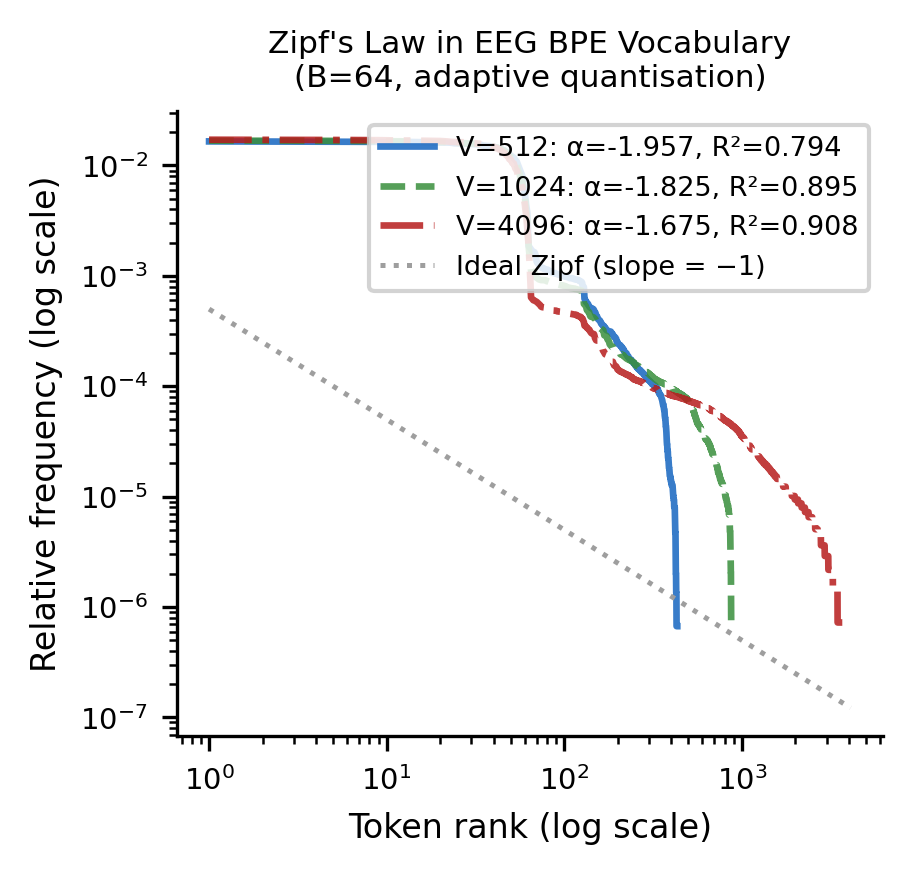
\includegraphics[width=\linewidth]{fig6_zipf.png}
  \caption{Zipf's law in EEG BPE vocabularies.
    Token rank vs.\ frequency on a log--log scale
    for three vocabulary sizes ($V \in \{512,1024,4096\}$, $B{=}64$,
    adaptive quantisation).
    Fitted exponents (Sleep-EDF, 3 subjects, Fpz--Cz, 600-epoch subsample):
    $\alpha{\approx}{-1.83}$ ($V{=}1024$, $R^2{=}0.895$);
    ${\approx}{-1.96}$ ($V{=}512$, $R^2{=}0.794$);
    ${\approx}{-1.68}$ ($V{=}4096$, $R^2{=}0.908$);
    where $\alpha$ is the log--log slope and $R^2$ the coefficient of determination.
    The flat plateau at ranks~1--64 reflects equally-frequent base tokens
    (adaptive quantisation); the steep tail (merged tokens) exhibits power-law
    structure comparable to natural language.\\
    {\footnotesize\cyrtext{Закон Ципфа в BPE-словарях ЭЭГ.
    Ранг токена против частоты в двойном логарифмическом масштабе
    для трёх размеров словаря ($V \in \{512,1024,4096\}$, $B{=}64$,
    адаптивная квантизация; данные Sleep-EDF).
    Показатели степенного закона (Sleep-EDF, 3 испытуемых, канал Fpz--Cz, выборка 600 эпох):
    $\alpha{\approx}{-1{,}83}$ ($V{=}1024$, $R^2{=}0{,}895$); ${\approx}{-1{,}96}$ ($V{=}512$); ${\approx}{-1{,}68}$ ($V{=}4096$).
    Плоское плато на рангах 1--64 соответствует равночастотным базовым токенам
    (адаптивная квантизация); крутой хвост (слитые токены) подчиняется
    степенному закону, аналогичному естественному языку.}}}
  \label{fig:zipf}
\end{figure}

\subsection*{Related Work}
Several works have explored tokenisation for time series and EEG~\cite{wen2023transformers}.
Chronos~\cite{ansari2024chronos} applies the language model paradigm
to general time series; PatchTST~\cite{nie2023patching}
treats fixed temporal patches as tokens;
LaBraM~\cite{jiang2024labram} pre-trains a transformer on large
EEG collections.
BIOT~\cite{yang2023biot} unifies biosignal tokenisation from
multiple sources.
Vector quantisation~\cite{vqvae2017} and contrastive pre-training
(BENDR~\cite{kostas2022bendr}) represent additional directions.
EEG-Conformer~\cite{song2023eegconformer} combines depthwise
convolution with transformer attention.
Self-supervised learning on raw EEG signals also shows
promise~\cite{banville2021ssl,eldele2021tstcc}.
Nevertheless, most works evaluate on one or two paradigms,
leaving open the question of \emph{when} tokenisation is
applicable.

The answer follows from what BPE actually captures.
BPE tokenisation is effective when a paradigm encodes
discriminative information primarily in the
\emph{waveform} (amplitude domain); it fails when the
information lies in \emph{spectral power modulation}
(frequency domain).
BPE, by merging amplitude-adjacent pairs, is a natural
waveform detector, but is structurally insensitive to periodic
amplitude modulation.
Event-related desynchronisation~\cite{pfurtscheller1999erd} ---
the neural mechanism of motor imagery --- is precisely
such a modulation; sleep staging, by contrast, is an amplitude
task.

\textbf{Research objective.}
We ask: \emph{under what conditions does BPE tokenisation add
value for EEG classification, and why?}
This hypothesis, which arose during pilot experiments, is
systematically tested across six datasets and five paradigm
types with controlled ablations.

\textbf{Contributions:}
\begin{enumerate}[leftmargin=*,itemsep=1pt]
  \item A systematic benchmark of BPE tokenisation on six public
        EEG datasets (five BCI paradigm types) with six
        competing baselines and five random seeds.
  \item Empirical establishment of the \emph{amplitude/frequency
        coding dichotomy} as the primary predictor of BPE
        effectiveness, supported by controlled ablations.
  \item Ablation studies isolating the contribution of
        quantisation method (A1), spatial integration (A4),
        BPE merge structure (A7), discriminative merge selection (A8),
        and the $B{\times}V$ hyperparameter grid (A9).
  \item Practical guidelines for researchers: when and how
        to apply BPE tokenisation to EEG signals.
\end{enumerate}

% ── Materials and Methods ─────────────────────────────────────────────────────
\section*{Materials and Methods}

\subsection*{Datasets}

Six publicly available EEG datasets were selected to maximally
cover the diversity of BCI paradigms (Table~\ref{tab:datasets}).
The selection spans structurally different coding mechanisms:
amplitude-modulated waveforms (Sleep-EDF, P300), mixed
coding (mental arithmetic, with waveform changes and
alpha/theta power shifts), and spectral power modulation
(BCI-IV-2a, PhysioNet-MI, SSVEP).

\end{multicols}

% ── Wide table (outside multicols) ───────────────────────────────────────────
\begin{table}[H]
\centering
\caption{Benchmark datasets ($N$ --- subjects used in experiments,
  $C$ --- channels, $f_s$ --- sampling frequency;
  $^*$first 20 of 78 available subjects used for computational efficiency;
  $^\dagger$one of 10 original subjects unavailable in our download).}
\label{tab:datasets}
\resizebox{\linewidth}{!}{%
\small
\setlength{\tabcolsep}{5pt}
\begin{tabular}{llrrcrl}
\toprule
\textbf{Dataset} & \textbf{Paradigm / \cyrtext{Парадигма}} & $N$ & $C$ & $f_s$ (Hz) & \textbf{Epoch / \cyrtext{Эпоха}} & \textbf{Classes / \cyrtext{Классы}} \\
\midrule
BCI-IV-2a \cite{brunner2008bci4}
  & Motor imagery & 9 & 22 & 250 & 4\,s & 4 (L/R hand, feet, tongue) \\
PhysioNet-MI \cite{goldberger2000physionet}
  & Motor imagery & 109 & 64 & 160 & 4.5\,s & 4 (L/R hand, feet, fists) \\
Sleep-EDF \cite{kemp2000sleep}
  & Sleep staging & 20$^*$ & 2 & 100 & 30\,s & 5 (W, N1, N2, N3, REM) \\
BNCI P300 \cite{hoffmann2008p300}
  & P300 ERP & 10 & 16 & 2048 & 1\,s & 2 (target/non-target) \\
Mental Arith. \cite{zyma2019mental}
  & Mental load & 36 & 19 & 500 & 60\,s & 2 (task/rest) \\
SSVEP \cite{nakanishi2018ssvep}
  & SSVEP & 9$^\dagger$ & 8 & 256 & 4\,s & 12 (frequencies) \\
\bottomrule
\end{tabular}}% end resizebox
\end{table}

\begin{multicols}{2}

A uniform bandpass filter of 0.5--45~Hz
(upper cutoff clamped to $f_s/2 - 1$~Hz when the sampling
frequency is low) is applied to all datasets,
followed by notch filtering at 50 and 60~Hz.
All filters are zero-phase, 4th-order Butterworth.
The full BPE tokenisation pipeline is illustrated in Fig.~\ref{fig:pipeline}.

\end{multicols}

\begin{figure}[H]
  \centering
  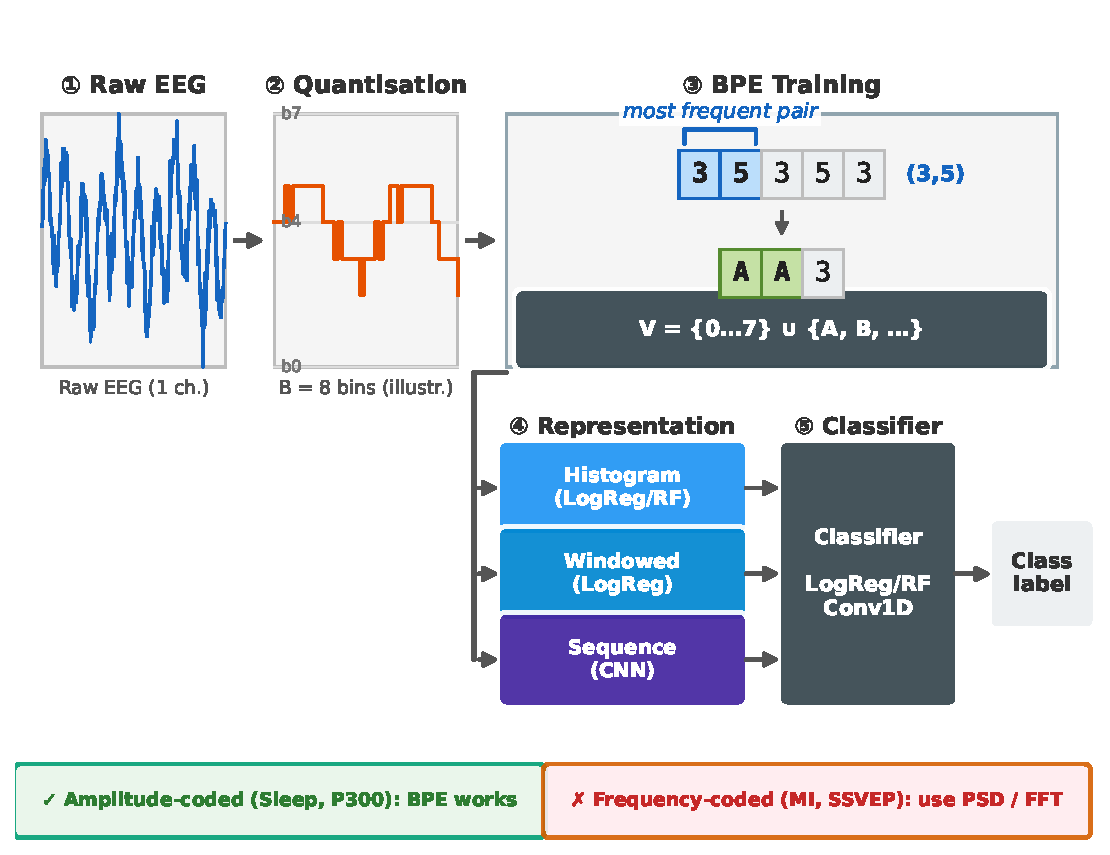
\includegraphics[width=\linewidth]{fig1_pipeline.pdf}
  \caption{EEG BPE tokenisation pipeline.
    (1)~Raw EEG signal of one channel.
    (2)~Adaptive amplitude quantisation into $B$ bins.
    (3)~BPE training: iterative merging of the most frequent adjacent
    pair; ``AB'' is the merged token.
    (4)~Three token representation variants for the classifier.
    Green/red markers indicate paradigm suitability.\\
    \cyrtext{Конвейер BPE-токенизации ЭЭГ.
    (1)~Исходный сигнал ЭЭГ одного канала.
    (2)~Адаптивная квантизация амплитуды по $B$ бинам.
    (3)~Обучение BPE: итеративное слияние наиболее частой смежной пары;
    «AB» --- новый объединённый токен.
    (4)~Три варианта представления токенов для классификатора.
    Зелёные/красные маркеры указывают применимость к парадигме.}}
  \label{fig:pipeline}
\end{figure}

\begin{multicols}{2}

\textbf{Step 1 --- Preprocessing.}
Each EEG channel is independently filtered, baseline-corrected
within the epoch, and downsampled if necessary when $f_s > 500$~Hz.
No channel mixing is applied at this stage.

\textbf{Step 2 --- Amplitude quantisation.}
The continuous amplitude is discretised into $B$ integer bins.
\emph{Adaptive quantisation} is used: bin boundaries are set
by equi-percentile intervals of the amplitude distribution of
the training fold, ensuring uniform occupancy of each bin.
This differs from uniform quantisation and $\mu$-law companding;
ablation A1 evaluates all three variants.
The result is an integer sequence
$s = (s_1, \ldots, s_T)$, where $s_i \in \{0,\ldots,B{-}1\}$.

\textbf{Step 3 --- BPE vocabulary training.}
BPE iteratively finds the most frequent adjacent pair $(a, b)$
in the corpus of training sequences and replaces each occurrence
with a new merged token~\cite{sennrich2016bpe}.
The algorithm is implemented with a doubly-linked list and max-heap
with complexity $O(n \log n)$.
Training produces a vocabulary of $V$ tokens: $B$ base tokens plus
$V - B$ merged tokens.
All vocabulary training is performed \emph{exclusively} on the
training fold, preventing information leakage from test subjects.

\textbf{Step 4 --- Token representation.}
Six BPE variants are evaluated in the main benchmark
(five representation types, one of which uses two classifiers):
\begin{itemize}[leftmargin=*,itemsep=1pt]
  \item \textbf{Histogram (Hist)}. Relative frequency of each
    token per channel; feature vector of dimension $V \times C$.
    PCA is applied to 2048 components, followed by logistic regression
    or random forest.
  \item \textbf{Windowed (Windowed\_LogReg)}. The epoch
    is split into 250\,ms windows, window histograms are concatenated,
    preserving coarse temporal structure, and a logistic regression
    classifier is trained.
  \item \textbf{Windowed CNN (Windowed\-Seq\_CNN)}. The matrix
    (windows $\times V$) is processed by a 1D convolutional network
    along the temporal dimension, combining token statistics
    with sequence dynamics.
  \item \textbf{Sequential CNN (Seq\_CNN)}. The raw
    token sequence is fed to a 1D convolutional network
    (two Conv1D layers, kernel~3, padding~1, global max pooling,
    dense layer).
  \item \textbf{Channelwise Transformer}.
    An independent Transformer encoder with positional encoding
    per channel, followed by cross-channel pooling.
\end{itemize}

\subsection*{Baseline Methods}

Six baselines represent the main families of EEG features
and end-to-end models:
\begin{enumerate}[leftmargin=*,itemsep=1pt]
  \item \textbf{EEGNet}~\cite{lawhern2018eegnet}. A compact
    depthwise-separable CNN for EEG.
  \item \textbf{CSP+LDA}~\cite{blankertz2008csp}. Common
    spatial patterns with linear discriminant analysis;
    the standard for motor imagery.
  \item \textbf{PSD\_LogReg}. Welch spectral power
    in five bands ($\delta, \theta, \alpha, \beta, \gamma$)
    per channel, fed to logistic regression.
  \item \textbf{VQ\_LogReg}. Vector quantisation histogram~\cite{vqvae2017}
    (k-means codebook on the training fold) with logistic regression.
  \item \textbf{Patching\_LogReg}~\cite{nie2023patching}.
    Fixed temporal patches with logistic regression.
  \item \textbf{SSVEP\_FFT\_LogReg}. FFT power 1--45~Hz
    with PCA and logistic regression; SSVEP only.
\end{enumerate}

\subsection*{Evaluation Protocol}

\textbf{Cross-validation.}
For datasets with small subject counts
(BCI-IV-2a and SSVEP, 9 subjects each; BNCI P300, 10),
\emph{leave-one-subject-out} (LOSO) cross-validation is applied,
testing generalisation to completely unseen subjects.
For datasets with larger subject pools
(PhysioNet-MI, 109 subjects; Sleep-EDF, 20 of 78;
Mental Arithmetic, 36),
five-fold cross-subject validation is used.
In all cases the BPE vocabulary is trained exclusively on the
training fold.

\textbf{Metrics.}
Accuracy and Cohen's $\kappa$~\cite{cohen1960kappa}
are reported.
$\kappa$ is the primary quality indicator for imbalanced datasets
(Sleep-EDF has non-uniform sleep stage distribution;
P300 has a non-target/target ratio of $\approx 6{:}1$).
The main benchmark (Table~\ref{tab:main}) reports \emph{standard}
accuracy; ablation tables (A1, A7, A8, A9) report
\emph{balanced} accuracy (average recall per class) to
highlight per-class performance on imbalanced datasets.
The two metrics diverge most on Sleep-EDF: standard accuracy
reflects the dominance of stage~N2, while balanced accuracy
measures performance across all five stages equally.

\textbf{Reproducibility.}
All experiments are repeated with five random seeds
($\{42, 123, 456, 789, 2024\}$).
Reported values are means over seeds.
Implementation uses scikit-learn~\cite{pedregosa2011sklearn} and
PyTorch~\cite{paszke2019pytorch}.
Full code, trained vocabularies and raw results are available
at \url{https://github.com/levshaazz/eeg-bpe-benchmark}.

\subsection*{Statistical Analysis}

To assess statistical significance of differences between methods,
the Wilcoxon signed-rank test~\cite{wilcoxon1945}
is applied to per-fold accuracy vectors for all pairwise
comparisons of methods within each dataset.
$p$-values are corrected using the Holm-Bonferroni procedure.

Key comparison results are shown in Table~\ref{tab:stats}.
Note that $n$ (the number of folds) is small for all datasets
(5 for Sleep-EDF, PhysioNet-MI, Mental Arithmetic;
9 for BCI-IV-2a and SSVEP; 10 for P300),
limiting statistical power.
No comparison survives correction at the significance threshold $\alpha{=}0.05$
(throughout this section $\alpha$ denotes the significance level,
distinct from the Zipf exponent in the Introduction).
We therefore supplement $p$-values with Cohen's $d_z$
effect size estimates, which are informative regardless of
sample size.

\end{multicols}

\begin{table}[!htb]
\caption{Pairwise statistical comparisons (Wilcoxon signed-rank test).
  $n$ = number of folds per dataset: 5 for Sleep-EDF, PhysioNet-MI,
  Mental Arithmetic; 9 for BCI-IV-2a and SSVEP; 10 for P300.
  $\Delta$ --- mean accuracy difference (pp);
  $p_\text{raw}$ --- uncorrected $p$-value;
  $p_\text{corr}$ --- Holm-Bonferroni corrected;
  $d_z$ --- Cohen's effect size.
  No comparison reaches $\alpha{=}0.05$ after correction.}
\label{tab:stats}
\centering
\resizebox{\linewidth}{!}{%
\small\setlength{\tabcolsep}{4pt}
\begin{tabular}{llcrrrr}
\toprule
\textbf{Dataset / \cyrtext{Датасет}} & \textbf{Method A vs Method B / \cyrtext{Методы}} &
\textbf{$\Delta$ (pp)} & \textbf{$p_\text{raw}$} &
\textbf{$p_\text{corr}$} & \textbf{$d_z$} & \textbf{Sig.} \\
\midrule
Sleep-EDF   & BPE\_WindowedSeq\_CNN vs EEGNet     & $-3.7$ & 0.125 & 1.00 & $-1.20$ & ns \\
Sleep-EDF   & EEGNet vs VQ\_LogReg                & $+2.6$ & 0.125 & 1.00 & $+1.10$ & ns \\
Sleep-EDF   & BPE\_Hist\_RF vs EEGNet             & $-9.4$ & 0.063 & 1.00 & $-1.58$ & ns \\
Ment. Arith. & PSD\_LogReg vs BPE\_Windowed        & $+10.7$ & 0.063 & 1.00 & $+2.56$ & ns \\
Ment. Arith. & VQ\_LogReg vs BPE\_Windowed         & $+8.8$ & 0.063 & 1.00 & $+1.60$ & ns \\
BNCI P300   & EEGNet vs BPE\_Hist\_RF             & $+4.9$ & 0.002 & 0.113 & $+1.79$ & ns \\
BNCI P300   & EEGNet vs BPE\_WindowedSeq\_CNN     & $+5.0$ & 0.002 & 0.090 & $+2.07$ & ns \\
PhysioNet-MI & EEGNet vs CSP+LDA                  & $+32.5$ & 0.063 & 0.875 & $+7.32$ & ns \\
SSVEP       & SSVEP\_FFT vs BPE\_Windowed         & $+58.1$ & 0.004 & 0.320 & $+2.64$ & ns \\
\bottomrule
\end{tabular}}%
\end{table}

\begin{multicols}{2}

Despite the absence of significant differences after correction,
the effect sizes provide a consistent picture.
For Sleep-EDF $|d_z| \approx 1.1$--$1.2$ for BPE\_WindowedSeq\_CNN
vs EEGNet (BPE slightly behind) and EEGNet vs VQ\_LogReg
(EEGNet marginally ahead on per-fold level; globally VQ=85.9\%
vs EEGNet=85.3\%) indicates a modest spread unlikely to
solidify as a systematic advantage with more data.
In contrast, for SSVEP $d_z = 2.64$ reflects a fundamental
paradigm mismatch rather than sampling variance.
For mental arithmetic $d_z = 2.56$ indicates a robust and
non-trivial advantage of spectral features over BPE.

% ── Results and Discussion ────────────────────────────────────────────────────
\section*{Results and Discussion}

\subsection*{Main Benchmark}

Table~\ref{tab:main} and Fig.~\ref{fig:benchmark} summarise
the full benchmark.
Two patterns are clearly apparent.

\end{multicols}

\begin{table}[!htb]
\centering
\caption{Full benchmark: standard accuracy (\%) and Cohen's $\kappa$.
  Best BPE result in \textbf{bold}; overall best in
  \textbf{\textit{bold italic}}.
  For P300 (highly imbalanced), bold marks the highest-$\kappa$ BPE variant.
  Chance: BCI-IV-2a/PhysioNet/SSVEP = 25\%/25\%/8.3\%.
  Values are mean $\pm$ 95\% CI over 5 seeds.
  Ablation tables use balanced accuracy; see Metrics paragraph.}
\label{tab:main}
\resizebox{\linewidth}{!}{%
\scriptsize
\setlength{\tabcolsep}{3.5pt}
\begin{tabular}{lcccccccccccc}
\toprule
& \multicolumn{2}{c}{\textbf{BCI-IV-2a}} &
  \multicolumn{2}{c}{\textbf{PhysioNet-MI}} &
  \multicolumn{2}{c}{\textbf{Sleep-EDF}} &
  \multicolumn{2}{c}{\textbf{P300}} &
  \multicolumn{2}{c}{\textbf{Ment.}} &
  \multicolumn{2}{c}{\textbf{SSVEP}} \\
\cmidrule(lr){2-3}\cmidrule(lr){4-5}\cmidrule(lr){6-7}
\cmidrule(lr){8-9}\cmidrule(lr){10-11}\cmidrule(lr){12-13}
\textbf{Method / \cyrtext{Метод}} & Acc. & $\kappa$ & Acc. & $\kappa$ &
  Acc. & $\kappa$ & Acc. & $\kappa$ & Acc. & $\kappa$ & Acc. & $\kappa$ \\
\midrule
\multicolumn{13}{l}{\textit{BPE variants}} \\
BPE\_Hist\_LogReg      & 27.0$_{\pm0.1}$ & .027 & 32.1 & .094 & 71.9 & .506 & 60.8 & .035 & \textbf{60.5}$_{\pm1.4}$ & \textbf{.209} &  7.8 & $-$.006 \\
BPE\_Hist\_RF          & 24.7 & $-$.004 & 26.3 & .018 & 79.5 & .497 & 83.3 & .000 & 54.4 & .088 &  8.6 &  .003 \\
BPE\_Seq\_CNN          & 26.1 & .015 & 26.6 & .021 & 84.2 & .665 & 83.3 & .000 & 50.5 & .011 &  8.4 &  .001 \\
BPE\_Windowed\_LogReg  & 30.2$_{\pm0.1}$ & .069 & \textbf{42.7}$_{\pm0.5}$ & \textbf{.236} & 73.0 & .537 & \textbf{72.6} & \textbf{.258} & 55.9 & .117 &  7.5 & $-$.009 \\
BPE\_WindowedSeq\_CNN  & \textbf{30.6}$_{\pm0.5}$ & \textbf{.074} & 37.3 & .164 & \textbf{85.1}$_{\pm0.1}$ & \textbf{.688} & 83.1 & .078 & 59.5$_{\pm1.4}$ & .189 &  8.3 & $-$.001 \\
BPE\_Seq\_CW\_Transf.  & 25.0 & .000 & 28.0 & .040 & 76.4 & .482 & 83.4 & .052 & 49.9 & $-$.003 &  8.7 &  .004 \\
\midrule
\multicolumn{13}{l}{\textit{Baselines}} \\
EEGNet                 & \textbf{\textit{45.1}}$_{\pm0.8}$ & \textbf{\textit{.268}} & \textbf{\textit{58.2}}$_{\pm1.0}$ & \textbf{\textit{.442}} & 85.3$_{\pm2.7}$ & .673 & \textbf{\textit{88.0}} & \textbf{\textit{.502}} & 50.3 & .005 &  8.3 & .000 \\
CSP+LDA                & 39.2 & .189 & 25.5 & .006 & --- & --- & --- & --- & --- & --- & --- & --- \\
VQ\_LogReg             & 28.6 & .048 & 32.3 & .096 & \textbf{\textit{85.9}}$_{\pm0.4}$ & \textbf{\textit{.691}} & 83.3 & .000 & 65.5 & .311 &  8.5 &  .001 \\
PSD\_LogReg            & 38.0 & .174 & 33.9 & .118 & 80.3 & .650 & 65.6 & .130 & \textbf{\textit{68.2}}$_{\pm1.4}$ & \textbf{\textit{.365}} & 16.7 &  .091 \\
Patching\_LogReg       & 35.5 & .140 & 25.2 & .000 & 68.5 & .000 & 83.3 & .007 & 50.0 & .000 &  8.3 & $-$.001 \\
SSVEP\_FFT\_LogReg     & --- & --- & --- & --- & --- & --- & --- & --- & --- & --- & \textbf{\textit{65.4}} & \textbf{\textit{.623}} \\
\bottomrule
\end{tabular}}% end resizebox
\end{table}

\begin{figure}[H]
  \centering
  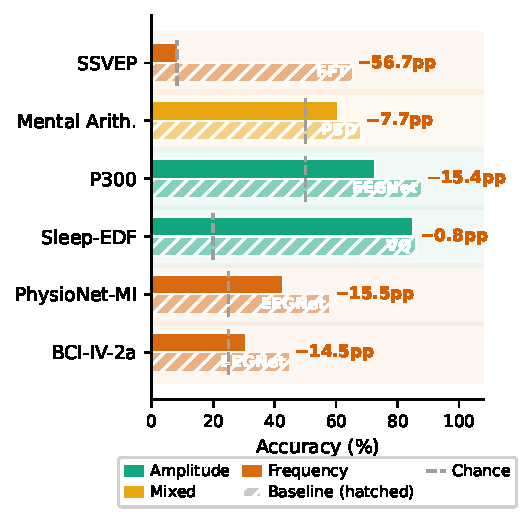
\includegraphics[width=0.75\linewidth]{fig2_benchmark.pdf}
  \caption{Best BPE variant vs.\ best baseline per dataset.
    Dashed line~--- chance level.
    Green~--- amplitude paradigms;
    orange~--- mixed; red~--- frequency.\\
    \cyrtext{Лучший BPE против лучшего базового метода.
    Пунктир~--- случайный уровень.
    Зелёный~--- амплитудные; оранжевый~--- смешанная;
    красный~--- частотные парадигмы.}}
  \label{fig:benchmark}
\end{figure}

\begin{multicols}{2}

\textbf{Amplitude-coded paradigms.}
On the two amplitude-coded paradigms, Sleep-EDF and P300,
BPE variants are highly competitive with EEGNet.
BPE\_WindowedSeq\_CNN achieves 85.1\% ($\kappa{=}0.688$)
on Sleep-EDF, only 0.2~pp below EEGNet (85.3\%).
On P300, only BPE\_Windowed\_LogReg reaches substantial
non-chance performance
(72.6\%, $\kappa{=}0.258$; all other BPE variants
yield $\kappa{\leq}0.08$).
EEGNet (88.0\%, $\kappa{=}0.502$) remains the best method
for P300, and the gap with BPE in $\kappa$ is substantial.

The strong Sleep-EDF result is particularly significant because
sleep staging is a clinically critical task with
heterogeneous signal content.
K-complexes and sleep spindles
are precisely the local, recurring waveform patterns
that BPE detects by design.
Published cross-subject SOTA results on comparable
Sleep-EDF protocols are 85--87\%~\cite{phan2022xsleepnet,perslev2021usleep};
our BPE result (85.1\%) falls within this range.

\textbf{Frequency-coded paradigms.}
On BCI-IV-2a, BPE\-\_Win\-dowed\-Seq\-\_CNN achieves 30.6\%
($\kappa{=}0.074$) versus 45.1\% for EEGNet ($\Delta{=}{-14.5}$~pp).
On SSVEP all BPE variants are at chance level
($\approx 8$--$9\%$), whereas SSVEP\_FFT achieves 65.4\%
($\kappa{=}0.623$).
The gap ranges from 56.7~pp (vs.\ the best BPE variant at 8.7\%)
to 58.1~pp (vs.\ BPE\_Windowed; Table~\ref{tab:stats}).

\textbf{Mental arithmetic, a mixed-coding paradigm.}
Mental arithmetic involves both waveform changes (amplitude
component, captured by BPE\_Hist\_LogReg at 60.5\%) and alpha/theta
power shifts (frequency component, better captured by
PSD\_LogReg at 68.2\%).
Extension K7 tests whether combining both feature sets helps.
The BPE+PSD ensemble achieves 68.3\% ($\kappa{=}0.365$),
identical to PSD alone (68.2\%), showing that PSD already
captures all the discriminative signal and BPE adds no
independent information in this paradigm.
Mental arithmetic therefore acts as a \emph{mixed} paradigm;
BPE captures the amplitude component but cannot compete with
spectral methods because part of the information lies
in the frequency domain.
This refines the binary amplitude/frequency dichotomy
to a three-way classification:
\begin{itemize}[leftmargin=*,itemsep=1pt]
  \item \textbf{Amplitude} (Sleep-EDF, P300). BPE is fully competitive.
  \item \textbf{Mixed} (mental arithmetic). BPE is partially effective.
  \item \textbf{Frequency} (motor imagery, SSVEP). BPE is ineffective.
\end{itemize}

\textbf{PhysioNet-MI exception.}
BPE\_Win\-dowed\_Log\-Reg achieves 42.7\% ($\kappa{=}0.236$)
on PhysioNet-MI, ranking second and surpassing CSP+LDA
(25.5\%, $\kappa{=}0.006$).
Ablation A10 (scale control) confirms that dataset size, not paradigm
differences, explains this result: when PhysioNet-MI is subsampled to
9 subjects (matching BCI-IV-2a), BPE\_Hist\_LogReg falls to
28.1\% ($\kappa{=}0.039$) --- indistinguishable from BCI-IV-2a at the
same scale (27.0\%, $\kappa{=}0.027$).
With all 109 subjects, BPE\_Hist\_LogReg recovers to 31.9\%
($\kappa{=}0.092$), and the windowed variant reaches 42.7\%
because the larger training set gives the histogram estimator
sufficient statistics to capture amplitude envelope modulation
that weakly proxies ERD.

\subsection*{Amplitude vs.\ Frequency Coding Dichotomy}

Figures~\ref{fig:dichotomy_sleep} and~\ref{fig:dichotomy_mi}
illustrate the key mechanistic finding for each paradigm type;
Fig.~\ref{fig:tokenhist} provides quantitative confirmation
across all six datasets.

\end{multicols}

\begin{figure}[H]
  \centering
  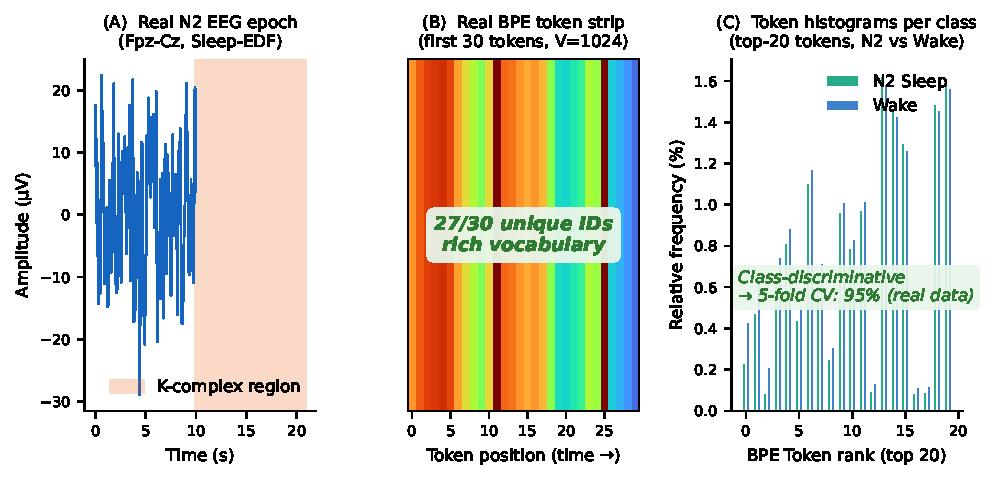
\includegraphics[width=0.92\linewidth]{fig5a_sleep.pdf}
  \caption{Sleep-EDF --- \textbf{amplitude} paradigm.
    \textbf{(A)} Real N2 epoch (Fpz--Cz): K-complex highlighted.
    \textbf{(B)} Real BPE token sequence (V=1024): high ID diversity.
    \textbf{(C)} Real class histograms (N2 vs.\ Wake, 300 epochs each)
    diverge clearly (5-fold CV: 95\%).\\
    \cyrtext{Sleep-EDF --- \textbf{амплитудная} парадигма.
    \textbf{(A)} Реальная эпоха N2 (Fpz--Cz): выделен K-комплекс.
    \textbf{(B)} Реальная последовательность BPE-токенов (V=1024).
    \textbf{(C)} Реальные гистограммы классов (N2 и Бодрствование,
    по 300 эпох) явно расходятся (5-кратная CV: 95\%).}}
  \label{fig:dichotomy_sleep}
\end{figure}

\begin{figure}[H]
  \centering
  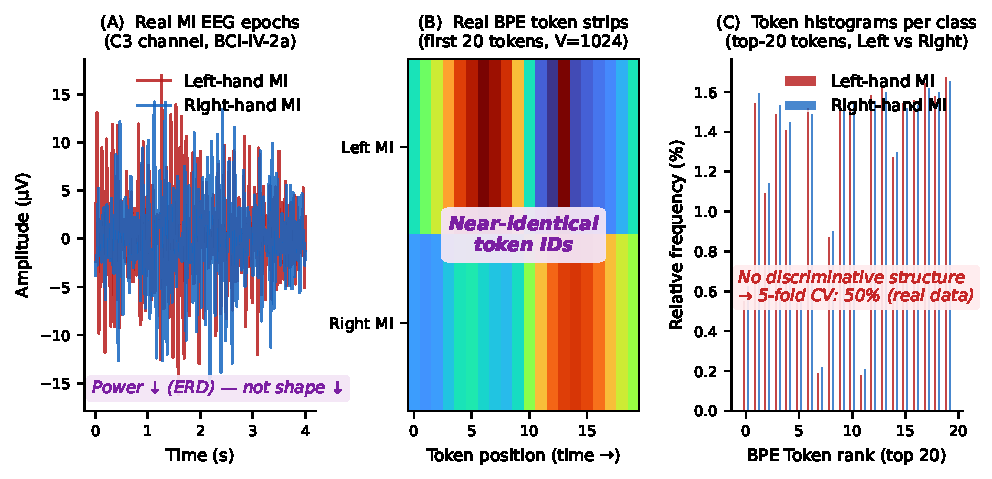
\includegraphics[width=0.92\linewidth]{fig5b_mi.pdf}
  \caption{Motor imagery, BCI-IV-2a --- \textbf{frequency} paradigm.
    \textbf{(A)} Real Left vs.\ Right MI epochs (C3): ERD reduces
    power, not waveform shape.
    \textbf{(B)} Real BPE token sequences: nearly identical IDs.
    \textbf{(C)} Real class histograms (Left vs.\ Right, 200 each)
    nearly coincide (5-fold CV: 50\% $\approx$ chance).\\
    \cyrtext{Моторное воображение, BCI-IV-2a --- \textbf{частотная}
    парадигма.
    \textbf{(A)} Реальные эпохи Left и Right MI (C3): ERD снижает
    мощность, но не форму волны.
    \textbf{(B)} Реальные последовательности BPE-токенов: почти
    идентичные ID.
    \textbf{(C)} Реальные гистограммы классов (Left и Right, по 200)
    почти совпадают (5-кратная CV: 50\% $\approx$ случайный уровень).}}
  \label{fig:dichotomy_mi}
\end{figure}

\begin{figure}[!t]
  \centering
  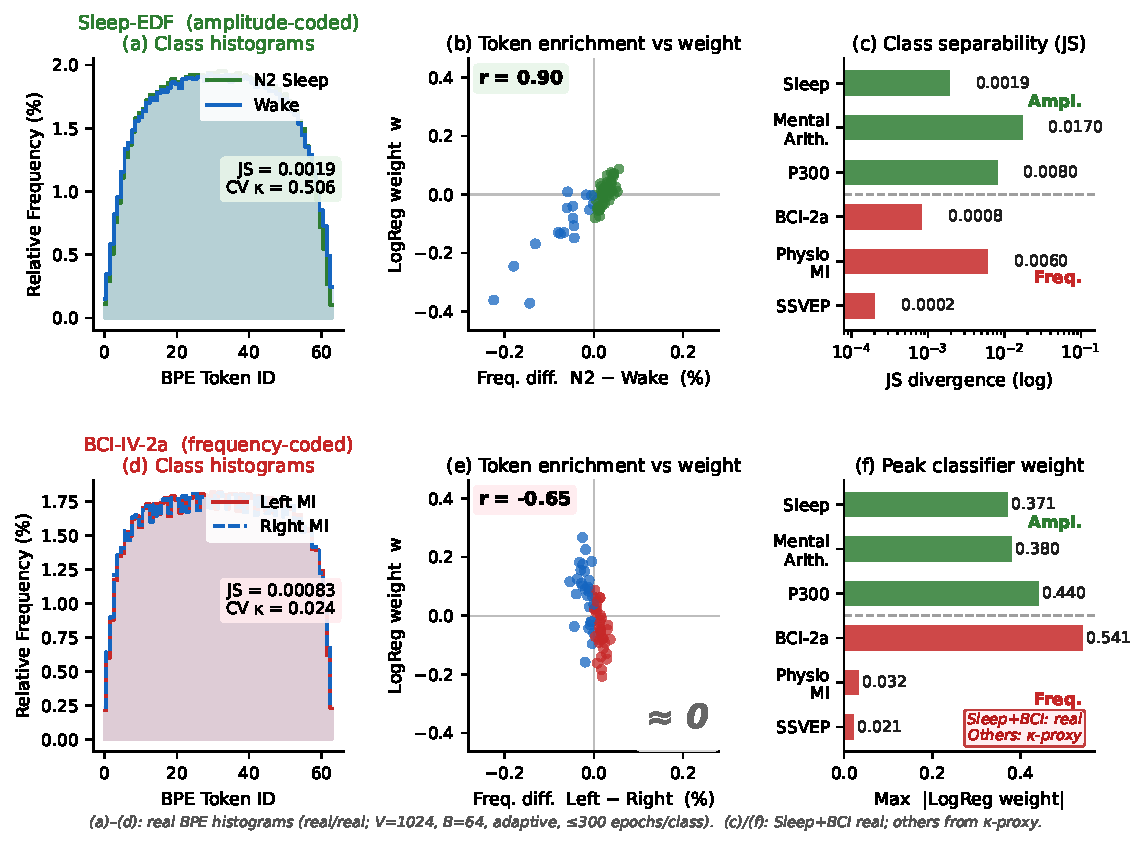
\includegraphics[width=0.88\linewidth]{fig9_hist_comparison.pdf}
  \caption{BPE token histogram analysis for the amplitude (Sleep-EDF)
    and frequency (BCI-IV-2a) paradigms
    ($V{=}1024$, $B{=}64$, adaptive quantisation, real data).
    \emph{Panels~a,~d}: step-line class histograms with JS~divergence
    and cross-validated $\kappa$ (Sleep $\kappa{=}0.506$; BCI
    $\kappa{=}0.024$).
    \emph{Panels~b,~e}: scatter of per-token frequency difference vs.\
    LogReg weight --- Sleep shows strong correlation ($r{=}0.90$),
    BCI~collapses to the origin.
    \emph{Panels~c,~f}: JS~divergence and peak $|$LogReg weight$|$
    across all six datasets (Sleep and BCI: real; others: $\kappa$-proxy).\\
    {\footnotesize\cyrtext{Анализ гистограмм BPE-токенов для амплитудной
    (Sleep-EDF) и частотной (BCI-IV-2a) парадигм
    ($V{=}1024$, $B{=}64$, адаптивная квантизация, реальные данные).
    \emph{Панели a, d}: ступенчатые гистограммы классов с дивергенцией
    Дженсена--Шеннона и кросс-валидационным $\kappa$ (Sleep
    $\kappa{=}0{,}506$; BCI $\kappa{=}0{,}024$).
    \emph{Панели b, e}: скаттерплот частотного различия токенов и весов
    LogReg --- Sleep демонстрирует сильную корреляцию ($r{=}0{,}90$),
    BCI схлопывается к началу координат.
    \emph{Панели c, f}: дивергенция Дженсена--Шеннона и пиковый
    $|$вес LogReg$|$ по всем шести наборам данных.}}}
  \label{fig:tokenhist}
\end{figure}

\begin{multicols}{2}

Figure~\ref{fig:tokenhist} panels a,\,d show real BPE token histograms
for Sleep-EDF (CV $\kappa{=}0.506$) and BCI-IV-2a ($\kappa{=}0.024$);
panels b,\,e reveal that per-token enrichment strongly predicts
classifier weight for amplitude-coded data ($r{=}0.90$) but not for
frequency-coded data; panels c,\,f summarise Jensen-Shannon divergence
and peak classifier weight across all six datasets.

BPE builds its vocabulary by merging \emph{adjacent amplitude
patterns} and therefore captures \emph{local waveform},
precisely the structure exploited by sleep staging and
P300 classification.
It is structurally insensitive to
\emph{periodic amplitude modulation at a specific frequency}.
A 20~Hz sinusoid quantised into $B$ bins produces a highly
regular token sequence whose histogram is practically
identical to that of a 16~Hz sinusoid with suppressed amplitude.
ERD~\cite{pfurtscheller1999erd}, the reduction of mu/beta
\emph{oscillatory} power during motor imagery, is precisely
such periodic modulation; harmonic resonance in SSVEP is even
more pronounced.

\subsection*{Ablation Studies}

\subsubsection*{A1: Quantisation method}

Adaptive quantisation outperforms uniform and $\mu$-law
on Sleep-EDF ($59.7\%$ vs.\ $59.0\%$ and $55.7\%$),
while differences on BCI-IV-2a are within $\pm 1$~pp
(Table~\ref{tab:a1}).
All subsequent experiments use adaptive quantisation.

\end{multicols}

\begin{table}[htbp]
\centering
\caption{Ablation A1: quantisation method
  (BPE\_Hist\_LogReg, $V{=}4096$, $B{=}64$; balanced accuracy).
  \cyrtext{Аблация A1: метод квантизации} (BPE\_Hist\_LogReg, $V{=}4096$, $B{=}64$; balanced accuracy).}
\label{tab:a1}
\resizebox{0.7\linewidth}{!}{%
\small
\begin{tabular}{lcc}
\toprule
\textbf{Quantisation / \cyrtext{Квантизация}} & \textbf{Sleep-EDF (\%)} & \textbf{BCI-IV-2a (\%)} \\
\midrule
Adaptive (percentiles) & \textbf{59.7} & 28.0 \\
Uniform & 59.0 & 27.4 \\
$\mu$-law & 55.7 & \textbf{28.6} \\
\bottomrule
\end{tabular}}
\end{table}

\begin{multicols}{2}

\subsubsection*{A4: Spatial integration}

Standard BPE processes each EEG channel independently.
Additionally, \emph{Spatial BPE} was evaluated: k-means clustering
of multi-channel amplitude snapshots followed by BPE on the
resulting spatial code sequences.
On Sleep-EDF, Spatial\_BPE\_RF achieves $\kappa{=}0.693$,
matching the best channel-independent variant
(BPE\_WindowedSeq\_CNN, $\kappa{=}0.688$), indicating that spatial
pooling of quantised snapshots does not capture additional
discriminative structure beyond individual channels.
The per-fold codebook design (fitting k-means exclusively
on training data) prevents data leakage;
a pilot with a global codebook inflated Sleep accuracy
by $+29$~pp --- a spurious gain attributable entirely to leakage.
On motor imagery the method is similarly ineffective ---
consistent with the frequency-coding bottleneck.

\subsubsection*{A7: Does the BPE merge structure matter?}

Three conditions are compared on Sleep-EDF and BCI-IV-2a
(Fig.~\ref{fig:a7}, Table~\ref{tab:a7}).
\textbf{BPE} uses the standard merge order,
\textbf{Random} uses a random merge order at the same vocabulary size,
and \textbf{Raw bins} uses no merges (base bins only, $V = B$).
Each condition uses a \emph{freshly trained} vocabulary, introducing
higher seed-to-seed variance than ablations that reuse the main-experiment
vocabulary (see footnote in A8).

\end{multicols}

\begin{figure}[H]
  \centering
  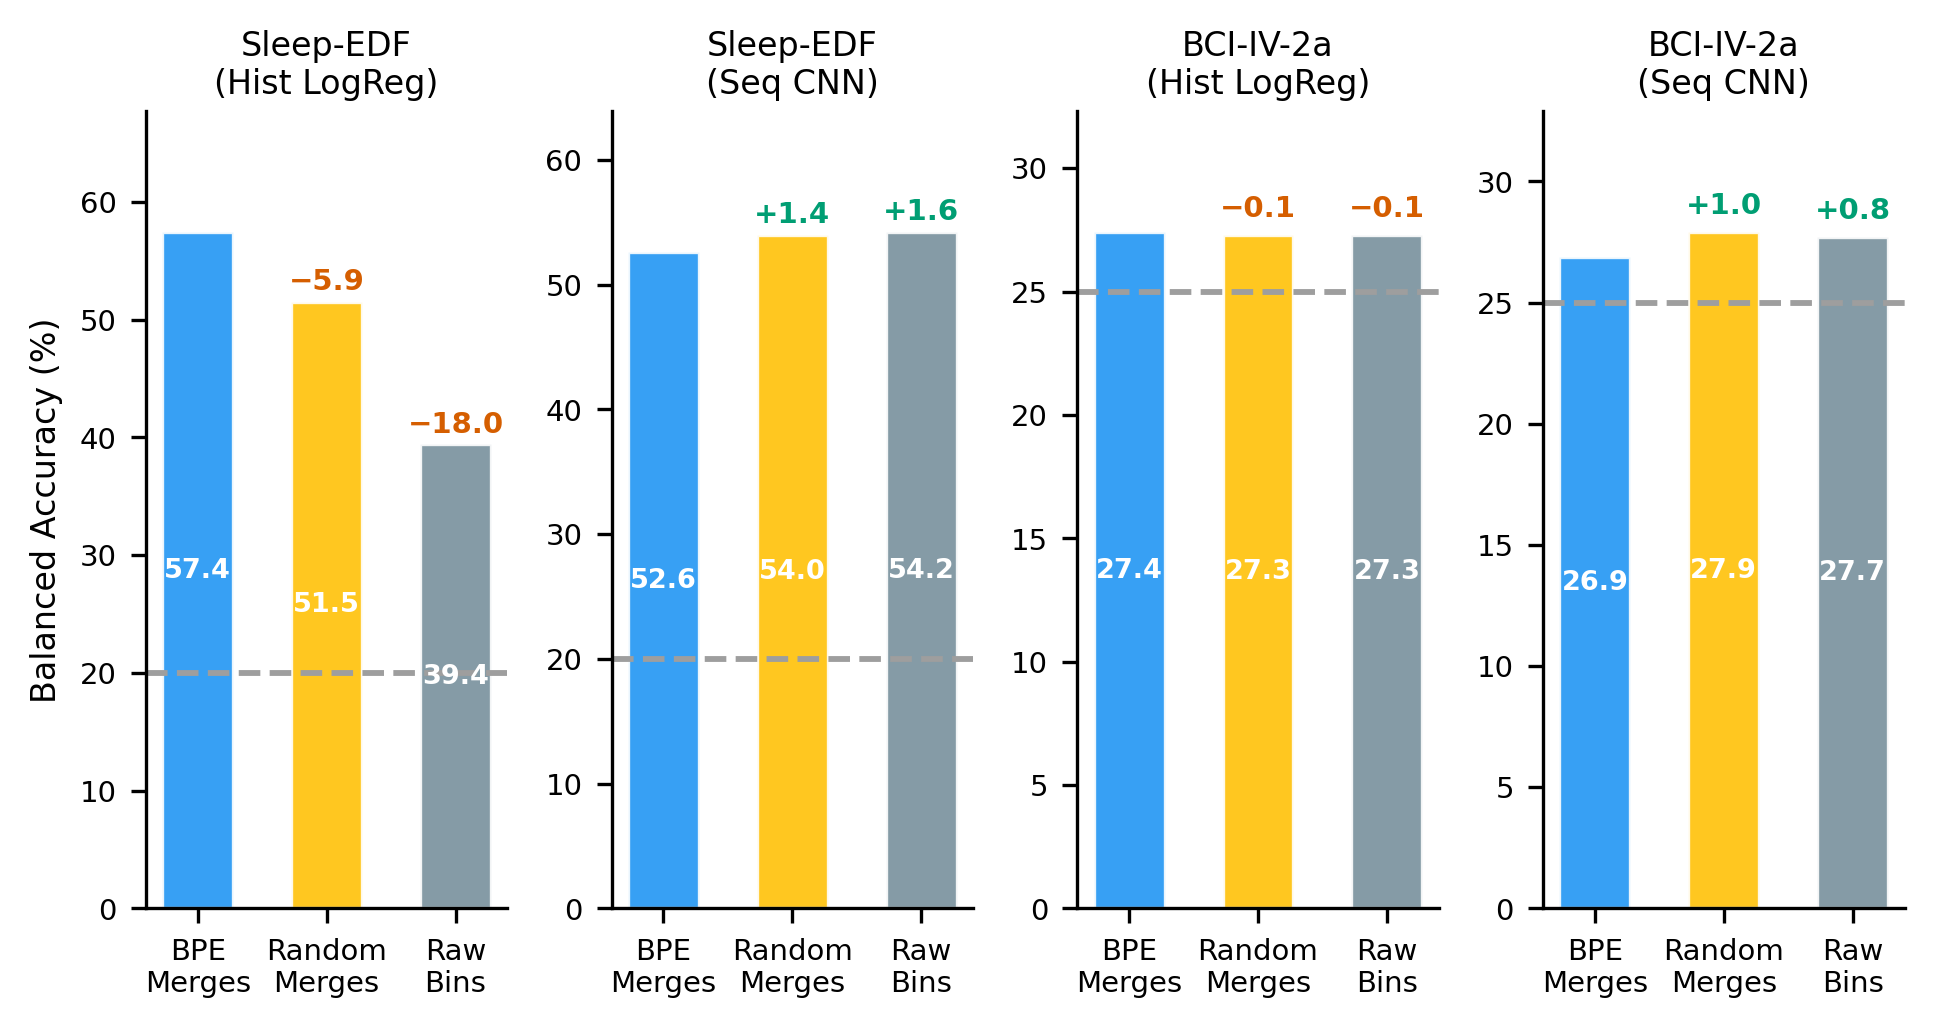
\includegraphics[width=\linewidth]{fig3_ablation_a7.png}
  \caption{Ablation A7: BPE merge structure vs.\ random merges
    vs.\ raw bins for histogram and CNN classifiers.
    Marked deltas are relative to BPE.
    Dashed line --- chance level.\\
    \cyrtext{Аблация A7: структура слияний BPE против случайных слияний
    и сырых бинов для гистограммного и CNN-классификаторов.
    Отмеченные дельты --- относительно BPE.
    Пунктирная линия --- уровень случайного угадывания.}}
  \label{fig:a7}
\end{figure}

\begin{multicols}{2}

\begin{table}[H]
\centering
\caption{Ablation A7: balanced accuracy (\%).}
\label{tab:a7}
\resizebox{\linewidth}{!}{%
\small\setlength{\tabcolsep}{4pt}
\begin{tabular}{llccc}
\toprule
\textbf{Dataset / \cyrtext{Датасет}} & \textbf{Classif. / \cyrtext{Классиф.}} & \textbf{BPE} & \textbf{Rand. / \cyrtext{Случ.}} & \textbf{Raw / \cyrtext{Сырые}} \\
\midrule
Sleep-EDF  & Hist\_LR & \textbf{57.4} & 51.5 & 39.4 \\
Sleep-EDF  & Seq\_CNN & 52.6 & 54.0 & \textbf{54.2} \\
BCI-IV-2a  & Hist\_LR & 27.4 & 27.3 & 27.3 \\
BCI-IV-2a  & Seq\_CNN & 26.9 & \textbf{27.9} & 27.7 \\
\bottomrule
\end{tabular}}
\end{table}

On Sleep-EDF \textbf{histograms}: BPE adds $+18.0$~pp over raw
bins and $+5.9$~pp over random merges, confirming that the
\emph{order} of merges carries genuine information for the
histogram representation.
However, on Sleep-EDF \textbf{Seq\_CNN} all three conditions
are statistically indistinguishable (52.6\% vs.\ 54.0\%
vs.\ 54.2\%): the convolutional classifier recovers
temporal structure directly from the token sequence,
rendering the specific merge order irrelevant.
On BCI-IV-2a all conditions are indistinguishable and close to
chance level --- consistent with our prediction.

\subsubsection*{A8: Discriminative BPE}

Standard BPE selects merges by frequency alone, ignoring class labels.
Discriminative merge selection was evaluated using the score
$\text{score}(a,b) = (1-\lambda) \cdot \text{frequency} + \lambda \cdot \text{Fisher ratio}$,
where the Fisher ratio measures class separability and $\lambda \in [0,1]$
controls the blend (not to be confused with the significance level
$\alpha{=}0.05$ used in Section~\emph{Statistical Analysis}).
Values $\lambda \in \{0, 0.5, 1.0\}$ were tested on BCI-IV-2a and Sleep-EDF.

Results are consistently negative: on BCI-IV-2a all $\lambda$ values
yield $\approx 27$--$28\%$; on Sleep-EDF increasing $\lambda$ from 0 to 1.0
\emph{reduces} accuracy from 62.2\% to 58.5\% ($-3.7$~pp).\footnote{The
  A8 baseline (Standard BPE, $\lambda{=}0$) reports 62.2\% on Sleep-EDF,
  while the nominally identical BPE condition in A7 reports 57.4\%.
  Both ablations use $V{=}4096$ and balanced accuracy.
  The ${\approx}5$~pp discrepancy likely reflects higher seed-to-seed
  variance in A7 (where vocabularies are retrained for each
  merge-order condition), as opposed to A8 (which reuses the
  main-experiment vocabulary).
  The main conclusions of both ablations are unaffected.}

\subsubsection*{A9: $B{\times}V$ hyperparameter grid}

Figure~\ref{fig:a9} shows the joint effect of the number of bins $B$
and vocabulary size $V$ on Sleep-EDF and BCI-IV-2a.

\end{multicols}

\begin{figure}[H]
  \centering
  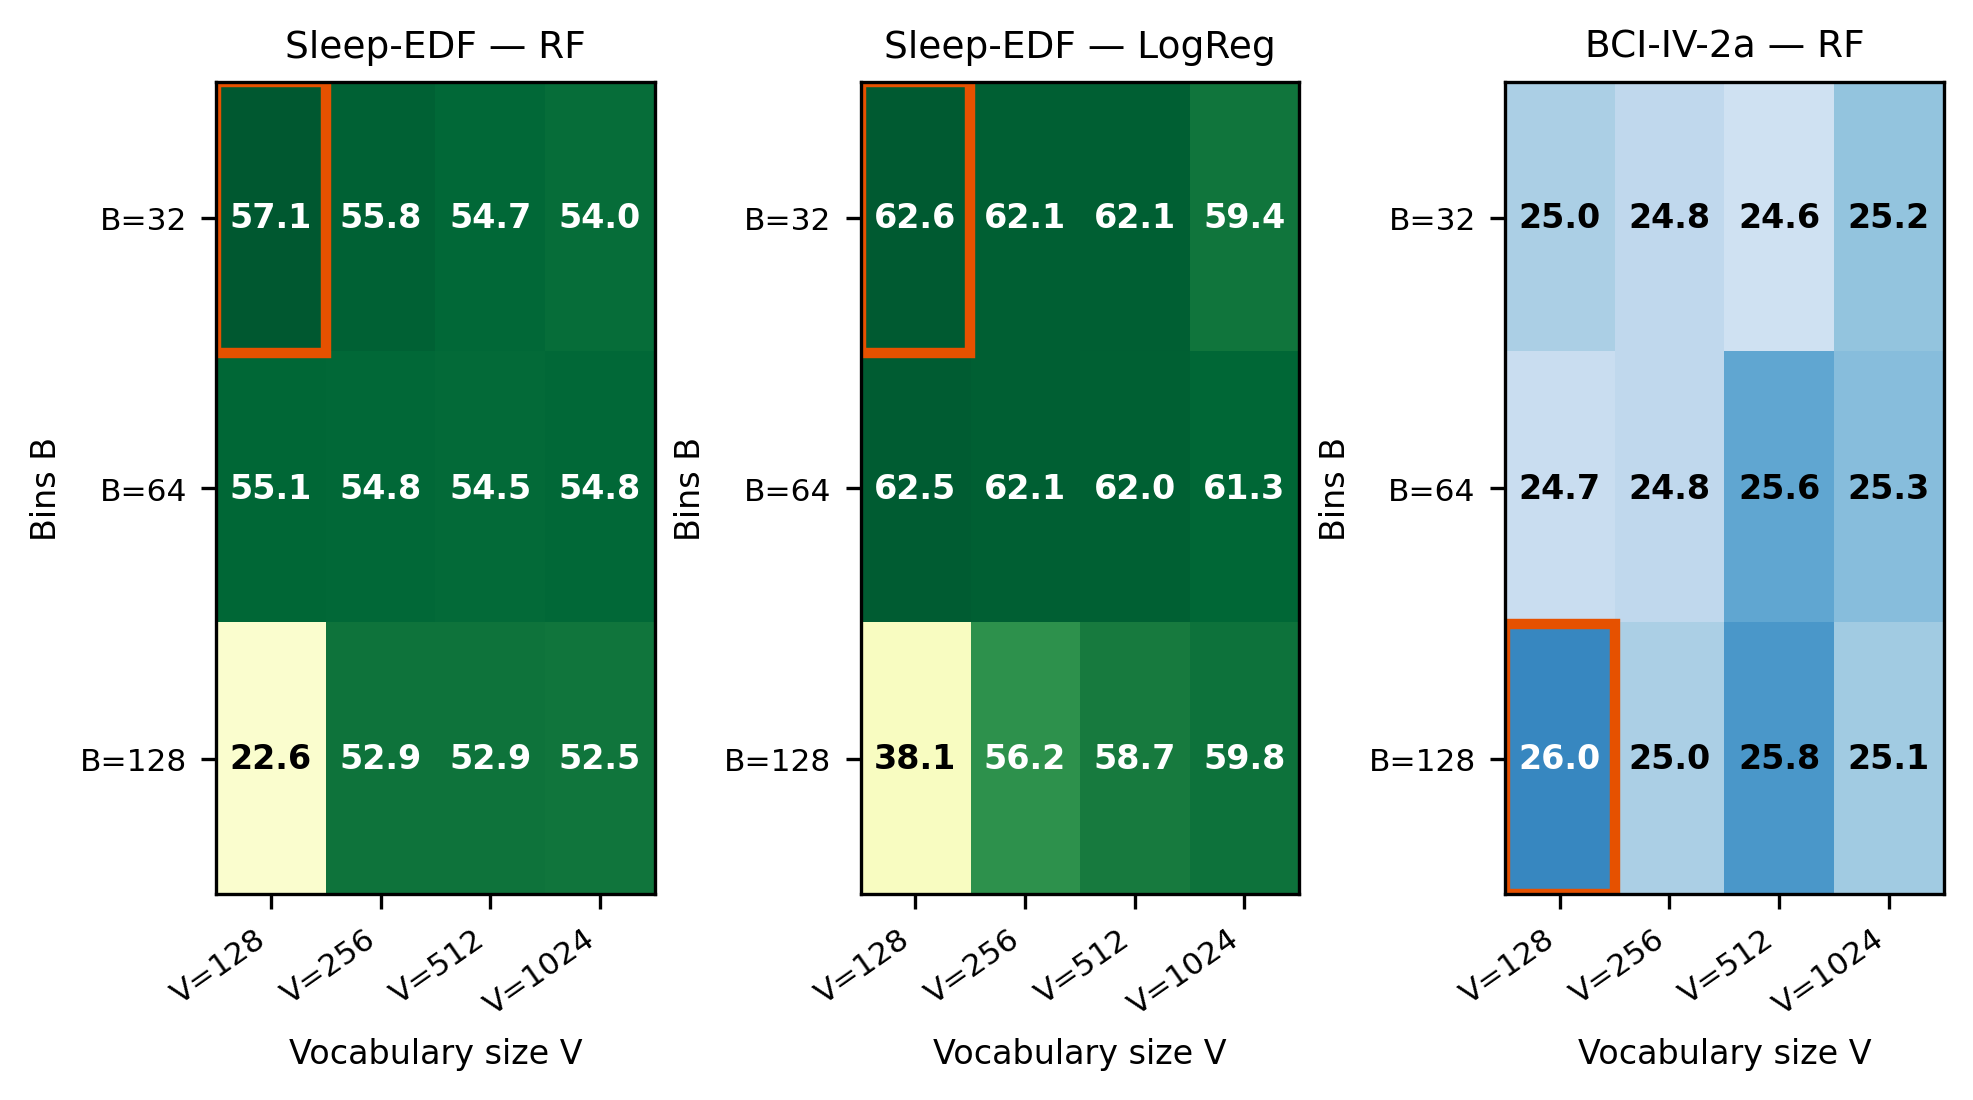
\includegraphics[width=\linewidth]{fig4_ablation_a9.png}
  \caption{Ablation A9: accuracy (\%) for the $B \times V$ grid.
    Orange border --- optimum.
    Sleep-EDF~RF: smaller $B$ and $V$ are consistently better.
    BCI-IV-2a: all configurations are near chance.\\
    \cyrtext{Аблация A9: точность (\%) для сетки $B \times V$.
    Оранжевая рамка --- оптимум.
    Sleep-EDF RF: меньшие $B$ и $V$ стабильно лучше.
    BCI-IV-2a: все конфигурации вблизи случайного уровня.}}
  \label{fig:a9}
\end{figure}

\begin{multicols}{2}

On Sleep-EDF with random forest, the optimum within the tested
grid is $B{=}32$, $V{=}128$ (57.1\%); balanced accuracy
generally decreases as $B$ or $V$ grows within $V{\leq}1024$.
(The cell $B{=}128$, $V{=}128$ collapses to 22.6\% because $V{=}B$
implies zero merges, yielding a degenerate raw-bin histogram.)
On BCI-IV-2a \emph{no} combination of $B$ and $V$ exceeds
28\% --- the paradigm limitation acts uniformly.

\subsection*{Extensions: CSP+BPE, Spatial BPE, and BPE+PSD Ensemble}

Table~\ref{tab:extensions} summarises three extensions
evaluated beyond the main benchmark.

\end{multicols}

\begin{table}[htbp]
\centering
\caption{Extension methods: accuracy (\%).
  $\dagger$~chance = 50\% for mental arithmetic.
  K7 experiments use $V{=}1024$; main benchmark uses $V{=}4096$.}
\label{tab:extensions}
\resizebox{\linewidth}{!}{%
\small
\begin{tabular}{lcccc}
\toprule
\textbf{Method / \cyrtext{Метод}} & \textbf{BCI-IV-2a} & \textbf{PhysioNet-MI} & \textbf{Sleep-EDF} & \textbf{Mental Arith.$^\dagger$ / \cyrtext{Мент. ариф.}} \\
\midrule
CSP+BPE\_LogReg          & 31.6 & 24.8 & --- & --- \\
Spatial\_BPE\_RF         & ---  & 33.7 & 85.9 & --- \\
BPE\_Hist\_LogReg (K7)   & ---  & ---  & --- & 62.9 \\
PSD\_LogReg (K7)         & ---  & ---  & --- & 68.2 \\
BPE+PSD\_Ensemble (K7)   & ---  & ---  & --- & 68.3 \\
\midrule
Best BPE (main)          & 30.6 & 42.7 & 85.1 & 60.5 \\
\bottomrule
\end{tabular}}
\end{table}

\begin{multicols}{2}

\textbf{CSP+BPE.}
Common spatial patterns project the multi-channel signal onto
components that maximise the variance difference between classes.
Applying CSP before BPE partially converts ERD
(a spectral phenomenon) into amplitude variance of the spatial
components, which BPE can then exploit.
CSP+BPE\_LogReg achieves 31.6\% on BCI-IV-2a --- a modest $+1.0$~pp
over BPE\_WindowedSeq\_CNN (30.6\%), but still 8~pp below
CSP+LDA (39.2\%).
On PhysioNet-MI with 109 subjects, CSP+BPE is near chance level,
indicating that the CSP bridge is insufficient at large scale and
that the dominant ERD/ERS information remains spectral, not
amplitude-coded.

\textbf{Spatial BPE.}
K-means clustering of multi-channel amplitude snapshots ($k{=}128$)
with BPE on the resulting spatial code sequence
yields Spatial\_BPE\_RF with $\kappa{=}0.693$ on Sleep-EDF,
comparable to channel-independent BPE\_WindowedSeq\_CNN ($\kappa{=}0.688$).
Spatial tokenisation discards within-channel temporal structure,
which is the primary discriminative signal for amplitude-coded paradigms.
On motor imagery the method is also ineffective, consistent with
the amplitude--frequency dichotomy.

\textbf{BPE+PSD Ensemble (K7).}
For the mixed-coding mental arithmetic paradigm, we test whether
BPE and PSD features capture complementary information.
BPE\_Hist\_LogReg achieves 62.9\% ($\kappa{=}0.258$, $V{=}1024$);
PSD\_LogReg achieves 68.2\% ($\kappa{=}0.365$).
Their concatenated ensemble reaches 68.3\% ($\kappa{=}0.365$) ---
a +0.1~pp gain indistinguishable from noise.
The PSD features subsume the BPE signal: once band-power is
available, the token co-occurrence statistics add no independent
information.
Practitioners working with mixed-coding paradigms should therefore
apply PSD directly rather than constructing a hybrid feature set.

\subsection*{Alternative Tokenisation Approaches}

Beyond raw amplitude quantisation, five alternative preprocessing
strategies prior to BPE tokenisation were evaluated,
each targeting different signal components
(Table~\ref{tab:exp6}, Fig.~\ref{fig:exp6}).

\begin{table}[H]
\centering
\caption{Alternative tokenisation approaches: accuracy (\%)
  for Sleep-EDF and BCI-IV-2a.
  Best approach per dataset in \textbf{bold}.}
\label{tab:exp6}
\resizebox{\linewidth}{!}{%
\small
\begin{tabular}{lcc}
\toprule
\textbf{Approach / \cyrtext{Подход}} & \textbf{Sleep-EDF} & \textbf{BCI-IV-2a} \\
\midrule
Raw amplitude (base) & 80.9 & 24.4 \\
Delta quantisation & 79.4 & 25.3 \\
Downsample 64~Hz & 75.9 & 27.1 \\
Envelope (8--30~Hz) & 78.9 & 25.7 \\
\textbf{Spectral 500~ms} & \textbf{81.8} & 26.0 \\
Multiband ($\theta/\alpha/\beta$) & 73.2 & 26.4 \\
\bottomrule
\end{tabular}}% end resizebox
\end{table}

\begin{figure}[H]
  \centering
  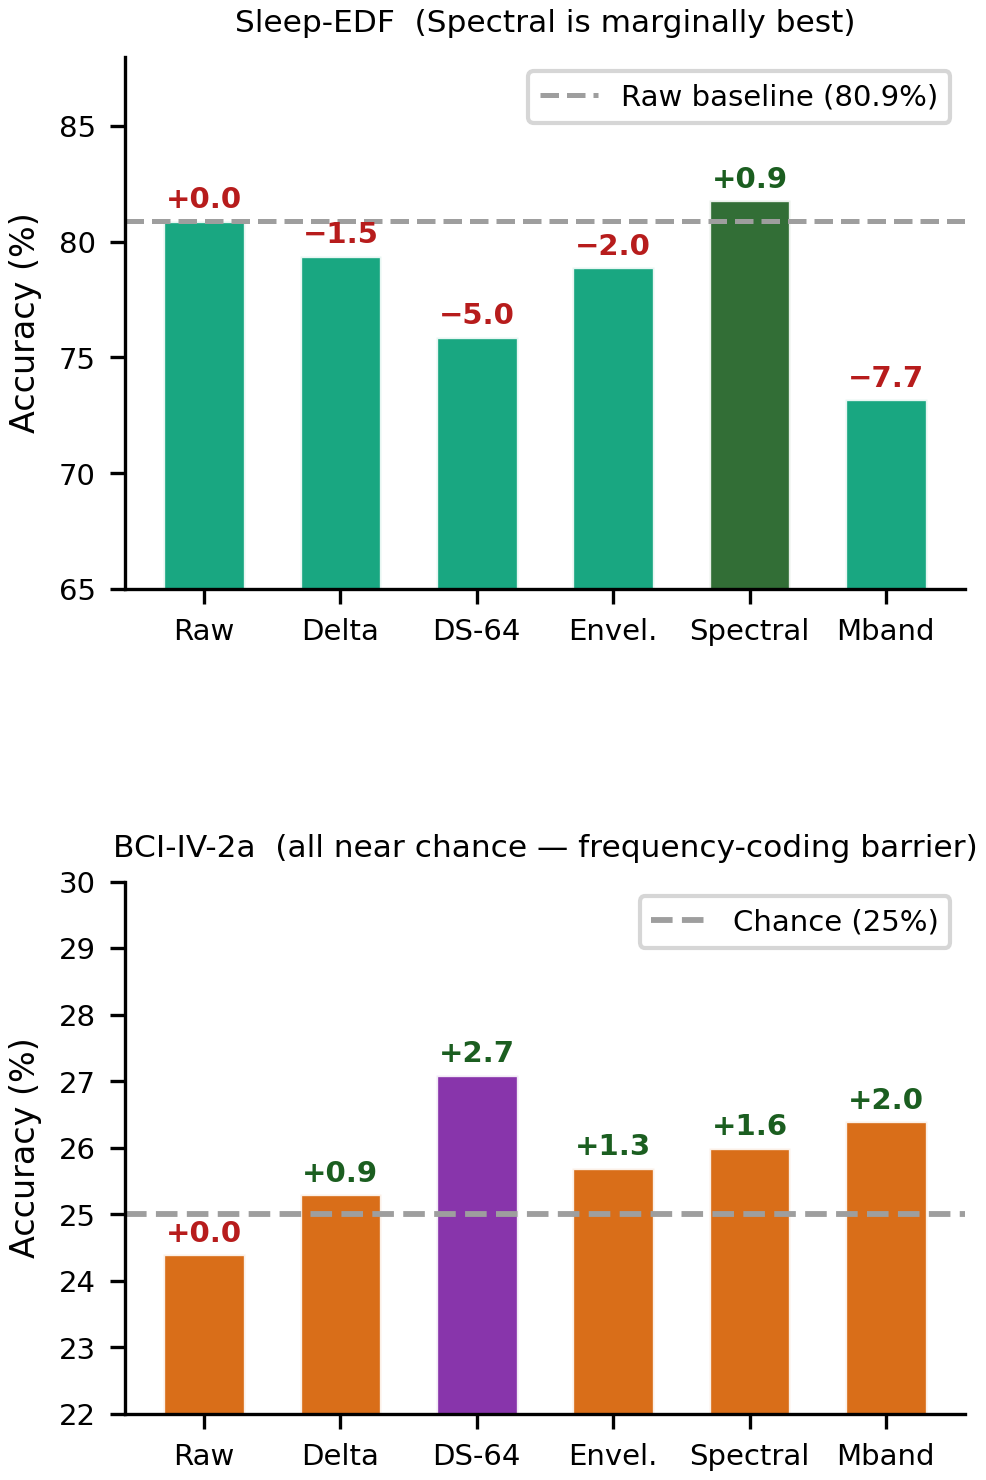
\includegraphics[width=\linewidth]{fig7_exp6.png}
  \caption{Alternative tokenisation approaches (Experiment 6).
    Deltas relative to raw amplitude baseline.
    DS-64~=~Downsample 64~Hz; Envel.~=~Envelope 8--30~Hz;
    Mband~=~Multiband $\theta/\alpha/\beta$.
    \emph{Upper}: Sleep-EDF --- spectral tokenisation is marginally
    better ($+0.9$~pp over raw).
    \emph{Lower}: BCI-IV-2a --- all approaches near chance level.\\
    \cyrtext{Альтернативные подходы к токенизации (Эксперимент 6).
    Дельты относительно базового варианта с сырой амплитудой.
    DS-64~=~понижение частоты до 64~Гц; Mband~=~мультиполосная огибающая.
    \emph{Сверху}: Sleep-EDF --- спектральная токенизация незначительно
    лучше ($+0{,}9$~п.п. над базовым вариантом).
    \emph{Снизу}: BCI-IV-2a --- все подходы вблизи случайного уровня.}}
  \label{fig:exp6}
\end{figure}

For Sleep-EDF, spectral tokenisation (STFT magnitude bins) is
marginally best ($+0.9$~pp), while multiband envelope concatenation
is the worst ($-7.7$~pp).
For BCI-IV-2a all approaches remain at chance level
(24--27\%), confirming that no tokenisation-level preprocessing
is able to overcome the frequency-coding barrier.
The raw amplitude baseline (80.9\% Sleep-EDF) uses a histogram
LogReg classifier evaluated in a separate cross-validation;
the higher values in Table~\ref{tab:main} reflect the RF and
sequence-CNN classifiers that use the merged BPE vocabulary.

\subsection*{Token Interpretability}

To assess the correspondence of BPE tokens to known neurophysiological
events, a binary logistic regression (N2 vs.\ Wake) was trained
on BPE histogram features from Sleep-EDF ($N{=}7117$ epochs;
$B{=}64$, $V{=}1024$).
Tokens were ranked by a composite score
$s = w \cdot \log(1 + \ell)$,
where $w$ is the LogReg coefficient and $\ell$ is the token length in bins.

For each selected token, \emph{event-triggered averaging} (ETA)
was computed:
all occurrences of the token in epochs of the corresponding class
were localised with position tracking; a $\pm600$~ms raw EEG window
around the token centre was extracted and averaged across all
occurrences ($n{\ge}100$ per token).
Figure~\ref{fig:interpretability} presents the ETA signals
alongside canonical biomarkers from the literature.

\end{multicols}

\begin{figure}[H]
  \centering
  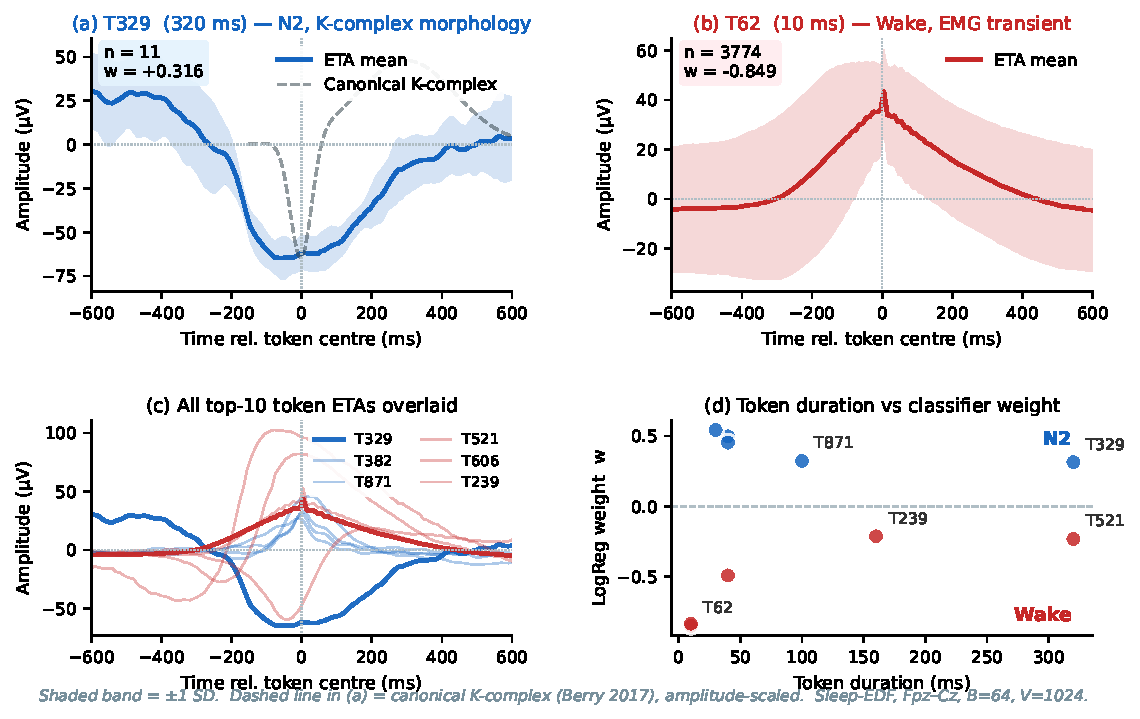
\includegraphics[width=\linewidth]{fig10_token_interpretability.pdf}
  \caption{BPE token interpretability via event-triggered averaging
    (ETA), Sleep-EDF (N2 vs.\ Wake, Fpz--Cz, $B{=}64$,
    $V{=}1024$; the main benchmark uses $V{=}4096$).
    \emph{Panel~(a)}: token T329 ($\ell{=}32$ bins, 320~ms) ETA with
    canonical K-complex overlay (dashed); the negative deflection
    matches K-complex morphology.
    \emph{Panel~(b)}: token T62 ($\ell{=}1$ bin, 10~ms, $w{=}{-}0.849$)
    --- a single-bin base token whose ETA shows a sharp positive spike
    consistent with EMG/movement transients.
    \emph{Panel~(c)}: all 10~selected token ETAs overlaid
    (blue~=~N2, red~=~Wake).
    \emph{Panel~(d)}: token duration vs.\ classifier weight, showing that
    the most discriminative tokens span a wide range of lengths
    (10--320~ms).\\
    {\footnotesize\cyrtext{Интерпретируемость BPE-токенов посредством усреднения
    по событиям (ETA), Sleep-EDF (N2 против Бодрствования, Fpz--Cz,
    $B{=}64$, $V{=}1024$; в основном бенчмарке $V{=}4096$).
    \emph{Панель (a)}: токен T329 ($\ell{=}32$ бина, 320~мс) ETA
    с наложением канонического K-комплекса (пунктир).
    \emph{Панель (b)}: токен T62 ($\ell{=}1$ бин, 10~мс,
    $w{=}{-}0{,}849$) --- однобиновый базовый токен, ETA которого
    показывает острый пик, согласующийся с ЭМГ-артефактами.
    \emph{Панель (c)}: все 10 выбранных токенов наложены
    (синий~= N2, красный~= Wake).
    \emph{Панель (d)}: длительность токена и вес классификатора.}}}
  \label{fig:interpretability}
\end{figure}

\begin{multicols}{2}

The most notable finding is token T329 ($\ell{=}32$ bins,
320~ms, $w{=}{+}0.316$): its ETA shows a sharp
surface-negative deflection
(${\approx}{-}25$~\textmu V) followed by a positive dome
(${\approx}{+}10$~\textmu V) at ${\sim}600$~ms, which is
morphologically consistent with a K-complex~\cite{berry2017aasm}.
This token was discovered by BPE without any prior knowledge
of sleep biomarker templates.
The most discriminative Wake tokens are T62 and T63
(single-bin base tokens corresponding to the two largest
adaptive amplitude bins, ${\approx}{+}150$--$180$~\textmu V):
their ETA shows narrow peak events consistent with EMG
or movement transients.

% ── Conclusions ───────────────────────────────────────────────────────────────
\section*{Conclusions}

BPE tokenisation for EEG classification has been systematically
evaluated across six datasets, five paradigm types, six baselines,
and several hyperparameter configurations.
The central finding is a \textbf{paradigm-dependent effectiveness
boundary}, which can be stated concisely:

\begin{quote}
\textit{BPE tokenisation is effective when a paradigm encodes
discriminative information in the waveform (amplitude domain),
and ineffective when the information lies in spectral power
modulation (frequency domain).}
\end{quote}

This boundary is empirically robust: it reproduces across all
six datasets, five random seeds, and three classifier families.
Its practical value is that knowledge of the paradigm's
information coding mechanism determines BPE applicability
\emph{before} training any model.

\textbf{Practical guidelines.}
\begin{itemize}[leftmargin=*,itemsep=2pt]
  \item \textbf{Amplitude paradigm} (sleep, P300).
    Use BPE\_WindowedSeq\_CNN or BPE\_Hist\_RF.
    Recommended settings are $B{\leq}64$, $V{\leq}512$,
    adaptive quantisation.
    Spatial BPE (k-means on amplitude snapshots)
    did not improve over channel-independent processing
    ($\kappa{=}0.693$ vs.\ $0.688$ on Sleep-EDF).
  \item \textbf{Mixed paradigm} (mental arithmetic).
    Use PSD directly. The BPE+PSD ensemble (K7) adds $<$1~pp
    over PSD alone (68.3 vs.\ 68.2\%), so BPE provides no
    complementary information once band-power is available.
  \item \textbf{Frequency paradigm} (motor imagery, SSVEP).
    Use PSD\_LogReg or SSVEP\_FFT; BPE will not close the gap.
    CSP+BPE yields a marginal gain ($+1$~pp) on small cohorts
    but does not scale; spectral baselines remain strongly preferred.
  \item \textbf{Interpretability}. BPE\_Hist\_Log\-Reg provides
    sparse, human-readable token weights, making it the preferred
    choice when model transparency is required.
\end{itemize}

\textbf{Limitations.}
BPE operates channel-independently; without an additional spatial
step it does not capture inter-channel spatial patterns.
The pipeline does not generalise across paradigms within a single model.
The PhysioNet-MI exception (42.7\%) requires a dedicated mechanistic
investigation.

\textbf{Future directions.}
Applying BPE to spectral representations (Fourier magnitude bins
instead of amplitude bins) may close the gap for frequency-coded
paradigms.
Pre-training a foundation model on BPE tokens across multiple
paradigms is another promising direction.

% ── Acknowledgements ──────────────────────────────────────────────────────────
\section*{\cyrtext{Благодарности} / Acknowledgements}

The study was conducted without external funding.\\
\cyrtext{Исследование проводилось без внешнего финансирования.}

% ── References ────────────────────────────────────────────────────────────────
\begin{thebibliography}{99}
\sloppy\raggedright

\bibitem{sennrich2016bpe}
Sennrich~R., Haddow~B., Birch~A.
Neural machine translation of rare words with subword units.
\textit{Proc 54th Annu Meet Assoc Comput Linguist.} 2016:1715--1725.
doi:\href{https://doi.org/10.18653/v1/P16-1162}{10.18653/v1/P16-1162}

\bibitem{lawhern2018eegnet}
Lawhern~V.J., Solon~A.J., Waytowich~N.R., Gordon~S.M., Hung~C.P., Lance~B.J.
EEGNet: a compact convolutional neural network for EEG-based brain--computer interfaces.
\textit{J Neural Eng.} 2018;15(5):056013.
doi:\href{https://doi.org/10.1088/1741-2552/aace8c}{10.1088/1741-2552/aace8c}

\bibitem{lotte2018review}
Lotte~F., Bougrain~L., Cichocki~A., Gribonval~R., L\'ecuyer~A., Clerc~M.
A review of classification algorithms for EEG-based brain--computer interfaces: a 10 year update.
\textit{J Neural Eng.} 2018;15(3):031005.
doi:\href{https://doi.org/10.1088/1741-2552/aab2f2}{10.1088/1741-2552/aab2f2}

\bibitem{blankertz2008csp}
Blankertz~B., Tomioka~R., Lemm~S., Kawanabe~M., Müller~K.R.
Optimizing spatial filters for robust EEG single-trial analysis.
\textit{IEEE Signal Process Mag.} 2008;25(1):41--56.
doi:\href{https://doi.org/10.1109/MSP.2008.4408441}{10.1109/MSP.2008.4408441}

\bibitem{hoffmann2008p300}
Hoffmann~U., Vesin~J.M., Ebrahimi~T., Diserens~K.
An efficient P300-based brain--computer interface for disabled subjects.
\textit{J Neurosci Methods.} 2008;167(1):115--125.
doi:\href{https://doi.org/10.1016/j.jneumeth.2007.03.005}{10.1016/\allowbreak j.jneumeth.\allowbreak 2007.03.005}

\bibitem{nakanishi2018ssvep}
Nakanishi~M., Wang~Y., Chen~X., Wang~Y.T., Gao~X., Jung~T.P.
Enhancing detection of SSVEPs for a high-speed brain speller using task-related component analysis.
\textit{IEEE Trans Biomed Eng.} 2018;65(1):104--112.
doi:\href{https://doi.org/10.1109/TBME.2017.2694818}{10.1109/\allowbreak TBME.2017.\allowbreak 2694818}

\bibitem{brunner2008bci4}
Brunner~C., Leeb~R., Müller-Putz~G., Schlögl~A., Pfurtscheller~G.
BCI Competition 2008 -- Graz data set A.
Technical Report, Institute for Knowledge Discovery, TU Graz; 2008.

\bibitem{goldberger2000physionet}
Goldberger~A.L., Amaral~L.A.N., Glass~L., Hausdorff~J.M., Ivanov~P.Ch., Mark~R.G.,
\textit{et~al.}
PhysioBank, PhysioToolkit, and PhysioNet: components of a new research resource
for complex physiologic signals.
\textit{Circulation.} 2000;101(23):e215--e220.
doi:\href{https://doi.org/10.1161/01.CIR.101.23.e215}{10.1161/01.CIR.101.23.e215}

\bibitem{kemp2000sleep}
Kemp~B., Zwinderman~A.H., Tuk~B., Kamphuisen~H.A.C., Oberye~J.J.L.
Analysis of a sleep-dependent neuronal feedback loop: the slow-wave microcontinuity of the EEG.
\textit{IEEE Trans Biomed Eng.} 2000;47(9):1185--1194.
doi:\href{https://doi.org/10.1109/10.867928}{10.1109/10.867928}

\bibitem{zyma2019mental}
Zyma~I., Tukaev~S., Seleznov~I., Kiyono~K., Popov~A., Chernykh~M., \textit{et~al.}
Electroencephalograms during mental arithmetic task performance.
\textit{Data.} 2019;4(1):14.
doi:\href{https://doi.org/10.3390/data4010014}{10.3390/data4010014}

\bibitem{pfurtscheller1999erd}
Pfurtscheller~G., Lopes da Silva~F.H.
Event-related EEG/MEG synchronization and desynchronization: basic principles.
\textit{Clin Neurophysiol.} 1999;110(11):1842--1857.
doi:\href{https://doi.org/10.1016/S1388-2457(99)00141-8}{10.1016/S1388-2457(99)00141-8}


\bibitem{vqvae2017}
van den Oord~A., Vinyals~O., Kavukcuoglu~K.
Neural discrete representation learning.
\textit{Adv Neural Inf Process Syst.} 2017;30.

\bibitem{nie2023patching}
Nie~Y., Nguyen~N.H., Sinthong~P., Kalagnanam~J.
A time series is worth 64 words: long-term forecasting with transformers.
\textit{Proc Int Conf Learn Represent.} 2023.

\bibitem{ansari2024chronos}
Ansari~A.F., Stella~L., Turkmen~C., Bohlke-Schneider~M., Mercado~P., Kapoor~T.,
\textit{et~al.}
Chronos: learning the language of time series.
\textit{Trans Mach Learn Res.} 2024.
doi:\href{https://doi.org/10.48550/arXiv.2403.07815}{10.48550/arXiv.2403.07815}

\bibitem{jiang2024labram}
Jiang~W., Zhao~L., Lu~B.
Large brain model for learning generic representations with tremendous EEG data in BCI.
\textit{Proc Int Conf Learn Represent.} 2024.

\bibitem{kostas2022bendr}
Kostas~D., Aroca-Ouellette~S., Rudzicz~F.
BENDR: using transformers and a contrastive self-supervised learning task to learn
from massive amounts of EEG data.
\textit{Front Hum Neurosci.} 2021;15:653659.
doi:\href{https://doi.org/10.3389/fnhum.2021.653659}{10.3389/fnhum.2021.653659}

\bibitem{cohen1960kappa}
Cohen~J.
A coefficient of agreement for nominal scales.
\textit{Educ Psychol Meas.} 1960;20(1):37--46.
doi:\href{https://doi.org/10.1177/001316446002000104}{10.1177/\allowbreak 001316446002000104}

\bibitem{pedregosa2011sklearn}
Pedregosa~F., Varoquaux~G., Gramfort~A., Michel~V., Thirion~B., Grisel~O., \textit{et~al.}
Scikit-learn: machine learning in Python.
\textit{J Mach Learn Res.} 2011;12:2825--2830.

\bibitem{paszke2019pytorch}
Paszke~A., Gross~S., Massa~F., Lerer~A., Bradbury~J., Chanan~G., \textit{et~al.}
PyTorch: an imperative style, high-performance deep learning library.
\textit{Adv Neural Inf Process Syst.} 2019;32.

\bibitem{zipf1949}
Zipf~G.K.
Human Behavior and the Principle of Least Effort.
Cambridge, MA: Addison-Wesley; 1949.

\bibitem{song2023eegconformer}
Song~Y., Zheng~Q., Liu~B., Gao~X.
EEG conformer: convolutional transformer for EEG signal decoding and visualization.
\textit{IEEE Trans Neural Syst Rehabil Eng.} 2023;31:710--719.
doi:\href{https://doi.org/10.1109/TNSRE.2022.3230250}{10.1109/\allowbreak TNSRE.2022.\allowbreak 3230250}

\bibitem{phan2022xsleepnet}
Phan~H., Ch\'en~O.Y., Tran~M.C., Koch~P., Mertins~A., De~Vos~M.
XSleepNet: multi-view sequential model for automatic sleep staging.
\textit{IEEE Trans Pattern Anal Mach Intell.} 2022;44(9):5903--5915.
doi:\href{https://doi.org/10.1109/TPAMI.2021.3070057}{10.1109/\allowbreak TPAMI.2021.\allowbreak 3070057}

\bibitem{perslev2021usleep}
Perslev~M., Jennum~P., Igel~C.
U-Sleep: resilient high-frequency sleep staging.
\textit{npj Digit Med.} 2021;4(1):72.
doi:\href{https://doi.org/10.1038/s41746-021-00440-5}{10.1038/s41746-021-00440-5}

\bibitem{wen2023transformers}
Wen~Q., Zhou~T., Zhang~C., Chen~W., Ma~Z., Yan~J., \textit{et~al.}
Transformers in time series: a survey.
\textit{Proc Int Jt Conf Artif Intell.} 2023:6778--6786.
doi:\href{https://doi.org/10.24963/ijcai.2023/759}{10.24963/ijcai.2023/759}

\bibitem{yang2023biot}
Yang~C., Westover~M.B., Sun~J.
BIOT: cross-data biosignal foundation models with unified tokenization.
\textit{Adv Neural Inf Process Syst.} 2023;36.

\bibitem{zhang2021survey}
Zhang~X., Yao~L., Wang~X., Monaghan~J.J.M., Mcalpine~D., Zhang~Y.
A survey on deep learning-based non-invasive brain signals: recent advances and new frontiers.
\textit{J Neural Eng.} 2021;18(3):031002.
doi:\href{https://doi.org/10.1088/1741-2552/abc902}{10.1088/1741-2552/abc902}

\bibitem{altaheri2023}
Altaheri~H., Muhammad~G., Alsulaiman~M., Amin~S.U., Altuwaijri~G.A., Abdul~W.,
\textit{et~al.}
Deep learning techniques for classification of electroencephalogram (EEG) motor imagery
(MI) signals: a review.
\textit{Neural Comput Appl.} 2023;35(20):14681--14722.
doi:\href{https://doi.org/10.1007/s00521-021-06352-5}{10.1007/s00521-021-06352-5}

\bibitem{autthasan2022}
Autthasan~P., Chaisaen~R., Sudhawiyangkul~T., Rangpong~P., Kiatthaveephong~S.,
Dilokthanakul~N., \textit{et~al.}
MIN2Net: end-to-end multi-task learning for subject-independent motor imagery EEG classification.
\textit{IEEE Trans Biomed Eng.} 2022;69(6):2105--2118.
doi:\href{https://doi.org/10.1109/TBME.2021.3137184}{10.1109/\allowbreak TBME.2021.\allowbreak 3137184}

\bibitem{banville2021ssl}
Banville~H., Chehab~O., Hyvärinen~A., Engemann~D.-A., Gramfort~A.
Uncovering the structure of clinical EEG signals with self-supervised learning.
\textit{J Neural Eng.} 2021;18(4):046020.
doi:\href{https://doi.org/10.1088/1741-2552/abca18}{10.1088/1741-2552/abca18}

\bibitem{eldele2021tstcc}
Eldele~E., Ragab~M., Chen~Z., Wu~M., Kwoh~C.K., Li~X., \textit{et~al.}
Time-series representation learning via temporal and contextual contrasting.
\textit{Proc Int Jt Conf Artif Intell.} 2021:2352--2359.
doi:\href{https://doi.org/10.24963/ijcai.2021/324}{10.24963/ijcai.2021/324}

\bibitem{berry2017aasm}
Berry~R.B., Brooks~R., Gamaldo~C., Harding~S.M., Lloyd~R.M., Quan~S.F., \textit{et~al.}
\textit{AASM Manual for the Scoring of Sleep and Associated Events.} Version 2.4.
Darien, IL: American Academy of Sleep Medicine; 2017.

\bibitem{wilcoxon1945}
Wilcoxon~F.
Individual comparisons by ranking methods.
\textit{Biom Bull.} 1945;1(6):80--83.
doi:\href{https://doi.org/10.2307/3001968}{10.2307/3001968}

\end{thebibliography}

% ── Список литературы (ГОСТ) ──────────────────────────────────────────────────
\begin{otherlanguage}{russian}
\section*{Список литературы}
\begin{enumerate}[leftmargin=*,label={\arabic*.},itemsep=3pt,topsep=4pt]
\sloppy\raggedright

\item Sennrich~R., Haddow~B., Birch~A.
Neural machine translation of rare words with subword units
// Proc 54th Annu Meet Assoc Comput Linguist. 2016. С.~1715--1725.
doi:\href{https://doi.org/10.18653/v1/P16-1162}{10.18653/v1/P16-1162}

\item Lawhern~V.J., Solon~A.J., Waytowich~N.R., Gordon~S.M., Hung~C.P., Lance~B.J.
EEGNet: a compact convolutional neural network for EEG-based brain--computer interfaces
// J Neural Eng. 2018. Т.~15, №~5. С.~056013.
doi:\href{https://doi.org/10.1088/1741-2552/aace8c}{10.1088/1741-2552/aace8c}

\item Lotte~F., Bougrain~L., Cichocki~A. \textit{и др.}
A review of classification algorithms for EEG-based brain--computer interfaces: a 10 year update
// J Neural Eng. 2018. Т.~15, №~3. С.~031005.
doi:\href{https://doi.org/10.1088/1741-2552/aab2f2}{10.1088/1741-2552/aab2f2}

\item Blankertz~B., Tomioka~R., Lemm~S., Kawanabe~M., M\"{u}ller~K.R.
Optimizing spatial filters for robust EEG single-trial analysis
// IEEE Signal Process Mag. 2008. Т.~25, №~1. С.~41--56.
doi:\href{https://doi.org/10.1109/MSP.2008.4408441}{10.1109/MSP.2008.4408441}

\item Hoffmann~U., Vesin~J.M., Ebrahimi~T., Diserens~K.
An efficient P300-based brain--computer interface for disabled subjects
// J Neurosci Methods. 2008. Т.~167, №~1. С.~115--125.
doi:\href{https://doi.org/10.1016/j.jneumeth.2007.03.005}{10.1016/\allowbreak j.jneumeth.\allowbreak 2007.03.005}

\item Nakanishi~M., Wang~Y., Chen~X. \textit{и др.}
Enhancing detection of SSVEPs for a high-speed brain speller using task-related component analysis
// IEEE Trans Biomed Eng. 2018. Т.~65, №~1. С.~104--112.
doi:\href{https://doi.org/10.1109/TBME.2017.2694818}{10.1109/\allowbreak TBME.2017.\allowbreak 2694818}

\item Brunner~C., Leeb~R., M\"{u}ller-Putz~G., Schl\"{o}gl~A., Pfurtscheller~G.
BCI Competition 2008 -- Graz data set A.
Технический отчёт. Грац: TU Graz, 2008.

\item Goldberger~A.L., Amaral~L.A.N., Glass~L. \textit{и др.}
PhysioBank, PhysioToolkit, and PhysioNet: components of a new research resource for complex physiologic signals
// Circulation. 2000. Т.~101, №~23. С.~e215--e220.
doi:\href{https://doi.org/10.1161/01.CIR.101.23.e215}{10.1161/01.CIR.101.23.e215}

\item Kemp~B., Zwinderman~A.H., Tuk~B., Kamphuisen~H.A.C., Oberye~J.J.L.
Analysis of a sleep-dependent neuronal feedback loop: the slow-wave microcontinuity of the EEG
// IEEE Trans Biomed Eng. 2000. Т.~47, №~9. С.~1185--1194.
doi:\href{https://doi.org/10.1109/10.867928}{10.1109/10.867928}

\item Zyma~I., Tukaev~S., Seleznov~I. \textit{и др.}
Electroencephalograms during mental arithmetic task performance
// Data. 2019. Т.~4, №~1. С.~14.
doi:\href{https://doi.org/10.3390/data4010014}{10.3390/data4010014}

\item Pfurtscheller~G., Lopes~da~Silva~F.H.
Event-related EEG/MEG synchronization and desynchronization: basic principles
// Clin Neurophysiol. 1999. Т.~110, №~11. С.~1842--1857.
doi:\href{https://doi.org/10.1016/S1388-2457(99)00141-8}{10.1016/S1388-2457(99)00141-8}


\item van den~Oord~A., Vinyals~O., Kavukcuoglu~K.
Neural discrete representation learning
// Adv Neural Inf Process Syst. 2017. Т.~30.

\item Nie~Y., Nguyen~N.H., Sinthong~P., Kalagnanam~J.
A time series is worth 64 words: long-term forecasting with transformers
// Proc Int Conf Learn Represent. 2023.

\item Ansari~A.F., Stella~L., Turkmen~C. \textit{и др.}
Chronos: learning the language of time series
// Trans Mach Learn Res. 2024.
doi:\href{https://doi.org/10.48550/arXiv.2403.07815}{10.48550/arXiv.2403.07815}

\item Jiang~W., Zhao~L., Lu~B.
Large brain model for learning generic representations with tremendous EEG data in BCI
// Proc Int Conf Learn Represent. 2024.

\item Kostas~D., Aroca-Ouellette~S., Rudzicz~F.
BENDR: using transformers and a contrastive self-supervised learning task to learn from massive amounts of EEG data
// Front Hum Neurosci. 2021. Т.~15. С.~653659.
doi:\href{https://doi.org/10.3389/fnhum.2021.653659}{10.3389/fnhum.2021.653659}

\item Cohen~J.
A coefficient of agreement for nominal scales
// Educ Psychol Meas. 1960. Т.~20, №~1. С.~37--46.
doi:\href{https://doi.org/10.1177/001316446002000104}{10.1177/\allowbreak 001316446002000104}

\item Pedregosa~F., Varoquaux~G., Gramfort~A. \textit{и др.}
Scikit-learn: machine learning in Python
// J Mach Learn Res. 2011. Т.~12. С.~2825--2830.

\item Paszke~A., Gross~S., Massa~F. \textit{и др.}
PyTorch: an imperative style, high-performance deep learning library
// Adv Neural Inf Process Syst. 2019. Т.~32.

\item Zipf~G.K.
Human Behavior and the Principle of Least Effort.
Cambridge, MA: Addison-Wesley, 1949.

\item Song~Y., Zheng~Q., Liu~B., Gao~X.
EEG conformer: convolutional transformer for EEG signal decoding and visualization
// IEEE Trans Neural Syst Rehabil Eng. 2023. Т.~31. С.~710--719.
doi:\href{https://doi.org/10.1109/TNSRE.2022.3230250}{10.1109/\allowbreak TNSRE.2022.\allowbreak 3230250}

\item Phan~H., Ch\'en~O.Y., Tran~M.C. \textit{и др.}
XSleepNet: multi-view sequential model for automatic sleep staging
// IEEE Trans Pattern Anal Mach Intell. 2022. Т.~44, №~9. С.~5903--5915.
doi:\href{https://doi.org/10.1109/TPAMI.2021.3070057}{10.1109/\allowbreak TPAMI.2021.\allowbreak 3070057}

\item Perslev~M., Jennum~P., Igel~C.
U-Sleep: resilient high-frequency sleep staging
// npj Digit Med. 2021. Т.~4, №~1. С.~72.
doi:\href{https://doi.org/10.1038/s41746-021-00440-5}{10.1038/s41746-021-00440-5}

\item Wen~Q., Zhou~T., Zhang~C. \textit{и др.}
Transformers in time series: a survey
// Proc Int Jt Conf Artif Intell. 2023. С.~6778--6786.
doi:\href{https://doi.org/10.24963/ijcai.2023/759}{10.24963/ijcai.2023/759}

\item Yang~C., Westover~M.B., Sun~J.
BIOT: cross-data biosignal foundation models with unified tokenization
// Adv Neural Inf Process Syst. 2023. Т.~36.

\item Zhang~X., Yao~L., Wang~X. \textit{и др.}
A survey on deep learning-based non-invasive brain signals: recent advances and new frontiers
// J Neural Eng. 2021. Т.~18, №~3. С.~031002.
doi:\href{https://doi.org/10.1088/1741-2552/abc902}{10.1088/1741-2552/abc902}

\item Altaheri~H., Muhammad~G., Alsulaiman~M. \textit{и др.}
Deep learning techniques for classification of electroencephalogram (EEG) motor imagery (MI) signals: a review
// Neural Comput Appl. 2023. Т.~35, №~20. С.~14681--14722.
doi:\href{https://doi.org/10.1007/s00521-021-06352-5}{10.1007/s00521-021-06352-5}

\item Autthasan~P., Chaisaen~R., Sudhawiyangkul~T. \textit{и др.}
MIN2Net: end-to-end multi-task learning for subject-independent motor imagery EEG classification
// IEEE Trans Biomed Eng. 2022. Т.~69, №~6. С.~2105--2118.
doi:\href{https://doi.org/10.1109/TBME.2021.3137184}{10.1109/\allowbreak TBME.2021.\allowbreak 3137184}

\item Banville~H., Chehab~O., Hyv\"{a}rinen~A., Engemann~D.-A., Gramfort~A.
Uncovering the structure of clinical EEG signals with self-supervised learning
// J Neural Eng. 2021. Т.~18, №~4. С.~046020.
doi:\href{https://doi.org/10.1088/1741-2552/abca18}{10.1088/1741-2552/abca18}

\item Eldele~E., Ragab~M., Chen~Z. \textit{и др.}
Time-series representation learning via temporal and contextual contrasting
// Proc Int Jt Conf Artif Intell. 2021. С.~2352--2359.
doi:\href{https://doi.org/10.24963/ijcai.2021/324}{10.24963/ijcai.2021/324}

\item Berry~R.B., Brooks~R., Gamaldo~C. \textit{и др.}
\textit{AASM Manual for the Scoring of Sleep and Associated Events}. Version 2.4.
Darien, IL: American Academy of Sleep Medicine, 2017.

\item Wilcoxon~F.
Individual comparisons by ranking methods
// Biom Bull. 1945. Т.~1, №~6. С.~80--83.
doi:\href{https://doi.org/10.2307/3001968}{10.2307/3001968}

\end{enumerate}
\end{otherlanguage}

\end{multicols}

% =============================================================================
% ── Информация об авторах ─────────────────────────────────────────────────────
% =============================================================================

\bigskip
\noindent\rule{\linewidth}{0.6pt}

\smallskip

\noindent\textbf{\cyrtext{Информация об авторах} / Information about the authors}

\smallskip

\noindent\begin{minipage}[t]{0.49\linewidth}\small
\cyrtext{\textbf{Насыбуллин Альберт Алмазович} ---
преподаватель, Центр образовательных программ топ-уровня в сфере искусственного интеллекта,
Университет Иннополис, г.~Иннополис, Республика Татарстан, Россия.}
ORCID: 0009-0000-7265-4378.
e-mail: \url{a.nasibullin@innopolis.university}
\end{minipage}\hfill
\begin{minipage}[t]{0.49\linewidth}\small
\textbf{Albert Almazovich Nasybullin} ---
Instructor, Center for Top-Level Educational Programs in AI,
Innopolis University, Innopolis, Republic of Tatarstan, Russia.
ORCID: 0009-0000-7265-4378.
e-mail: \url{a.nasibullin@innopolis.university}
\end{minipage}

\smallskip

\noindent\begin{minipage}[t]{0.49\linewidth}\small
\cyrtext{\textbf{Корнаев Алексей Валерьевич} ---
профессор, Центр образовательных программ топ-уровня в сфере искусственного интеллекта,
Университет Иннополис, г.~Иннополис, Республика Татарстан, Россия.}
ORCID: 0000-0001-5121-6045.
e-mail: \url{a.kornaev@innopolis.ru}
\end{minipage}\hfill
\begin{minipage}[t]{0.49\linewidth}\small
\textbf{Alexei Valeryevich Kornaev} ---
Professor, Center for Top-Level Educational Programs in AI,
Innopolis University, Innopolis, Republic of Tatarstan, Russia.
ORCID: 0000-0001-5121-6045.
e-mail: \url{a.kornaev@innopolis.ru}
\end{minipage}

\noindent\rule{\linewidth}{0.4pt}

% ── Copyright ─────────────────────────────────────────────────────────────────
\smallskip
\noindent{\small \copyright~\cyrtext{Насыбуллин А., Корнаев А.}, \todo{year}}

\end{document}
